%% LyX 2.1.5 created this file.  For more info, see http://www.lyx.org/.
%% Do not edit unless you really know what you are doing.
\documentclass[letterpaper,english,10pt]{bmc_template/bmcart}
\usepackage{mathptmx}
\usepackage[T1]{fontenc}
\usepackage[latin9]{inputenc}
\usepackage{array}
\usepackage{float}
\usepackage{units}
\usepackage{amsmath}
\usepackage{amssymb}
\usepackage[dvips]{graphicx}
\usepackage{setspace}
\usepackage{wasysym}
\usepackage{nomencl}
% the following is useful when we have the old nomencl.sty package
\providecommand{\printnomenclature}{\printglossary}
\providecommand{\makenomenclature}{\makeglossary}
\makenomenclature
\doublespacing

\makeatletter

%%%%%%%%%%%%%%%%%%%%%%%%%%%%%% LyX specific LaTeX commands.
\special{papersize=\the\paperwidth,\the\paperheight}

%% Because html converters don't know tabularnewline
\providecommand{\tabularnewline}{\\}
%% A simple dot to overcome graphicx limitations
\newcommand{\lyxdot}{.}

\floatstyle{ruled}
\newfloat{algorithm}{tbp}{loa}
\providecommand{\algorithmname}{Algorithm}
\floatname{algorithm}{\protect\algorithmname}

%%%%%%%%%%%%%%%%%%%%%%%%%%%%%% User specified LaTeX commands.
\usepackage{babel}

\usepackage{cite}
\usepackage{color}
\usepackage{bigdelim,multirow}
\usepackage{tikz}
\usetikzlibrary[arrows,calc,decorations.pathmorphing,backgrounds,positioning,fit,petri,shapes,decorations.markings]
\usepackage{pgfplots}
\usepackage{babel}
\usepackage{multirow}

\usepackage{algpseudocode}
\usepackage{algorithm}

\usepackage{nicefrac}

\usepackage{setspace}

\renewcommand{\algorithmicrequire}{\textbf{Input:}}
\renewcommand{\algorithmicensure}{\textbf{Output:}}

%\newcolumntype{L}[1]{>{\raggedright\let\newline\\\arraybackslash\hspace{0pt}}m{#1}}
%\newcolumntype{C}[1]{>{\centering\let\newline\\\arraybackslash\hspace{0pt}}m{#1}}
%\newcolumntype{R}[1]{>{\raggedleft\let\newline\\\arraybackslash\hspace{0pt}}m{#1}}

% unnumbered footnote
\makeatletter
\newcommand{\unfootnote}[1]{
  \renewcommand{\@makefnmark}{}
  \footnotetext{#1}
  \renewcommand{\@makefnmark}{\mbox{$^{\@thefnmark}$}}
}
\makeatother

\newcommand{\jj}{\operatorname{j}}      % imaginary unit

\makeatother

\usepackage{babel}
\begin{document}
\begin{frontmatter}

\begin{fmbox}
\dochead{Research Article}

\title{Design of Adaptive Constellations and Error Protection Coding for
Wireless Network Coding in 5-node Butterfly Networks}

\author[
   addressref={aff1},
   email={pavel@prochazka.info}
]{\inits{PP}\fnm{Pavel} \snm{Prochazka}}
\author[
   addressref={aff1},
   email={uricatom@fel.cvut.cz}
]{\inits{TU}\fnm{Tomas} \snm{Uricar}}
\author[
   addressref={aff2},                   % id's of addresses, e.g. {aff1,aff2}
   corref={aff2},                       % id of corresponding address, if any
   %noteref={n1},                        % id's of article notes, if any
   email={david.halls@toshiba-trel.com}   % email address
]{\inits{DH}\fnm{David} \snm{Halls}}
\author[
   addressref={aff1},
   email={jan.sykora@fel.cvut.cz}
]{\inits{JS}\fnm{Jan} \snm{Sykora}}


\address[id=aff1]{%                           % unique id
  \orgname{Czech Technical University in Prague}, % university, etc
  \street{Technicka 2},                     %
  \postcode{16627}                                % post or zip code
  \city{Prague},                              % city
  \cny{CZ}                                    % country
}
\address[id=aff2]{%
  \orgname{Toshiba -- Telecommunication Research Laboratory},
  \street{32 Queen Square},
  \postcode{BS1 4ND}
  \city{Bristol,},
  \cny{UK}
}
\end{fmbox}% comment this for two column layout


\begin{abstractbox}

\begin{abstract} % abstract
In this paper we focus on the design of a reliable communication scheme
for generic 5-node Wireless Butterfly Networks (WBN). Since the WBN
represents a natural extension of the basic 2-way relay communication
channel, we follow the paradigm of \emph{Wireless Physical Layer Network
Coding} and we show that the design of novel adaptive constellations\emph{
} is desirable to exploit the promising performance of wireless network coding in WBN.
We introduce a \emph{systematic constellation design} algorithm and
we show that the proposed constellations are capable of outperforming
conventional point-to-point modulations in WBN over the whole range
of channel signal to noise ratios. To further support the applicability of the proposed
constellations in a practical system, we integrate a simple binary
channel coding scheme, providing a robust \emph{adaptive modulation
and coding scheme} for relaying in symmetric WBNs with arbitrary channel
conditions.
\end{abstract}

\begin{keyword}
\kwd{wireless network coding}
\kwd{butterfly network}
\kwd{relaying}
\kwd{superposition coding}
\kwd{superposition modulation}
\end{keyword}

% MSC classifications codes, if any
%\begin{keyword}[class=AMS]
%\kwd[Primary ]{}
%\kwd{}
%\kwd[; secondary ]{}
%\end{keyword}

\end{abstractbox}


\end{frontmatter}






\section{Introduction}

The invention of Wireless Network Coding\emph{ }(WNC) has indeed provided
a means for a significant enhancement in wireless system performance
\cite{Popovski-Yomo_2007a,Nazer-Gastpar_2011-IEEE-P,Zhang-Liew-Lu_2012}.
However, WNC processing has also revealed several non-trivial research
problems which do not have counterparts in conventional point-to-point
or multi-user systems, like the sensitivity to channel parameterization
\cite{Koike-Popovski-Tarokh_2008,Liu-Tao-Xu_2011-ICC,Yasami-Razi-Abedi_2011,Uricar-Sykora_2011}
or challenging multi-source transmission synchronization \cite{Zhang-Liew-Lam_2006b-ITW,Rosetto-Zorzi_2009-SPAWC,Huang-Wang-Song-Guo-Jamalipour_2012-IEEE-T-WC}.
Furthermore, the specific characteristics of multi-node WNC systems
can call also for novel constellation design approaches (see e.g.
\cite{Uricar-Sykora_2011,Prochazka-Uricar-Halls-Sykora_2015-ICC}).

In WNC the transmitted information symbols are allowed to interact
directly in the constellation space, inducing a specific set of requirements
on the constellations' properties and characteristics (see e.g. \cite{Uricar-Sykora_2011,Prochazka-Uricar-Halls-Sykora_2015-ICC}).
Generally we can declare \cite{Prochazka-Uricar-Halls-Sykora_2015-ICC}
that any constellation suitable for the specific nature of WNC processing
should be able to form\emph{ a superimposed constellation} with an
appropriate structure at all receiving nodes (allowing direct decoding
of specific WNC functions of user data from the received non-orthogonal
signals \cite{Nazer-Gastpar_2008-ISIT,Sykora-Burr_2011-TVT}) and
simultaneously it should be able to exploit the \emph{broadcast nature
}of wireless channels (allowing a reduction in the consumption of
channel resources in the system \cite{Popovski-Yomo_2007a}). Since
both of these properties hinge on the actual SNR conditions in the
system, the constellation design itself can become a relatively challenging
task.


One of the first attempts to design a suitable multi-source constellation
for communication in a multi-node WNC system was introduced in our
previous work \cite{Prochazka-Uricar-Halls-Sykora_2015-ICC}, where
the \emph{adaptive 2-source constellations} for WNC-based communication
in a 5-node \emph{Wireless Butterfly Network} (WBN) were developed.
However, the results presented in \cite{Prochazka-Uricar-Halls-Sykora_2015-ICC}
are limited to an uncoded system, which significantly limits its practical
applicability. 

In this paper we extend the communication scheme from \cite{Prochazka-Uricar-Halls-Sykora_2015-ICC}
by appending appropriate \emph{error protection coding} to the system,
resulting in a practical channel-coded adaptive communication scheme
for WBN. We provide the following results and contributions:
\begin{enumerate}
\item We summarize the \emph{systematic constellation design algorithm}
from \cite{Prochazka-Uricar-Halls-Sykora_2015-ICC} and we provide
additional numerical results analysing its promising performance.
\item We revise and extend the results discussing the \emph{adaptive capabilities
of the constellations, }including \emph{the constellation mapping
regions} for adaptive WBN relaying\emph{.}
\item We validate the proposed design in a \emph{real-world HW setup}, including
the HW evaluation of adaptive system performance.
\item We show how the \emph{channel coding} can be integrated into the proposed
constellation design, including the analysis of proper source transmission
rates.
\item We evaluate numerically the performance of the resulting \emph{adaptive
modulation and coding} scheme for a wide range of channel conditions
in the WBN.
\item We show that the proposed design is viable even if the real-world
conditions induce some deviation from the assumed system model.
\end{enumerate}
The rest of the paper is organized as follows. The system model, including
all necessary definitions and details about WNC processing in WBNs
is summarized in Section~\ref{sec:CTUpp_SystemModel}. A systematic
\emph{constellation design algorithm} for WBNs is revised in Section~\ref{sec:CTUpp_Euclidean-Distance-based-Constel}.
The performance analysis of the proposed constellations (including
the HW evaluation) in an uncoded system is available in Section~\ref{sec:CTUpp_Performance-Analysis-Uncoded}.
Section~\ref{sec:CTUpp_Adaptive-Constellation-Design} discusses
an adaptive constellation design and Section~\ref{sec:CTUpp_Channel-Coding}
introduces the channel coding extension to the system. The performance
of the novel adaptive modulation and coding scheme is analyzed in
Section~\ref{sec:CTUpp_Performance-Analysis-Coded}, including a
simple robustness analyzis. Concluding remarks are summarized in Section~\ref{sec:CTUpp_DiscussionConclusions-etc}.


\section{WNC Relaying in Wireless Butterfly Network\label{sec:CTUpp_SystemModel}}

We assume a \emph{symmetric} WBN model \cite{Uricar-Qian-Sykora-Mow_2013-WCNC,Uricar-Qian-Sykora-Mow_2014-IEEE-T-WC}
with a half-duplex constraint (Fig. \ref{fig:CTUpp_Information_flows}).
An example practical scenario complying with the WBN model is a communication
among vehicles and road-side infrastructure nodes for traffic information
exchange on a bidirectional highway within two time slots \cite{Ho-Liew-Lu}.
The direct channels between the intended source$\rightarrow$destination
pairs are not available in WBN and thus the help of the intermediate
relay node is necessary to enable end-to-end communication. Please
note that in this paper we do not limit our attention to the above
mentioned special example of a high-speed, vehicle-based WBN.


\subsection{Relaying Strategy}

An information-theoretic relaying strategy (based on Superposition
Coding (SC) \cite{Cover-Thomas_ElemInfTheory,Han-Kobayashi_1981,Shende-Rajan-2012-NCC,Popovski-Carvalho_2008})
for WBNs was proposed in \cite{Uricar-Qian-Sykora-Mow_2013-WCNC,Uricar-Qian-Sykora-Mow_2014-IEEE-T-WC}.
The fundamental idea of the SC-approach is to split each data symbol
$\mathbf{d}_{i}$ at source $i\in\left\{ A,B\right\} $ into the \emph{basic
part} $\mathbf{d}_{i}^{b}=[d_{i,0}^{b},\dots,d_{i,N_{b}-1}^{b}]$
and the \emph{superposed part} $\mathbf{d}_{i}^{s}=[d_{i,0}^{s},\dots,d_{i,N_{s}-1}^{s}]$,
$d_{i,n}^{b},\,d_{i,n}^{s}\in\left\{ 0,1\right\} $, and then process
each of the resulting data streams separately throughout the system
(see Fig. \ref{fig:CTUpp_Information_flows}). While the basic part
represents a \textquotedbl{}true WNC\textquotedbl{} information stream
(limited by the amount of available HSI) in the system, the superposed
part defines the \textquotedbl{}routed\textquotedbl{} information
which is appended on top of the WNC stream to exploit any potential
spare capacity of related channels in the system (see \cite{Uricar-Qian-Sykora-Mow_2013-WCNC,Uricar-Qian-Sykora-Mow_2014-IEEE-T-WC}
for more details). A simplified description of SC-based relaying in
an uncoded WBN system is summarized in Table~\ref{tab:CTUpp_SC-relaying-scheme}
and depicted in Fig.~\ref{fig:CTUpp_Information-flow-uncoded-block-scheme}.
\begin{table}
\centering{}%
\begin{tabular}{|>{\raggedright}p{0.95\columnwidth}|}
\hline 
\textbf{Step 1: Source transmission}
\begin{itemize}
\item Source $S_{i},\,i\in\left\{ A,B\right\} $ maps its data symbol $\mathbf{d}_{i}=\left[\mathbf{d}_{i}^{b};\mathbf{d}_{i}^{s}\right]$
into a $\left(N_{b}+N_{s}\right)$-bit superposition modulation symbol
\begin{equation}
s_{i}=\mathcal{A}^{i}\left(\left[\mathbf{d}_{i}^{b};\mathbf{d}_{i}^{s}\right]\right),\label{eq:CTUpp_OverallSourceStreams}
\end{equation}

\item $S_{A},\,S_{B}$ simultaneously transmit their signals to the relay
and unintended destinations (Fig.~\ref{fig:CTUpp_Information_flows}).
\item Relay receives
\begin{equation}
x=h_{AR}\mathcal{A}^{A}\left(\left[\mathbf{d}_{A}^{b};\mathbf{d}_{A}^{s}\right]\right)+h_{BR}\mathcal{A}^{B}\left(\left[\mathbf{d}_{B}^{b};\mathbf{d}_{B}^{s}\right]\right)+w_{R}
\end{equation}



and decodes $\left[\mathbf{d}_{A}^{s};\mathbf{d}_{B}^{s};f(\mathbf{d}_{A}^{b},\mathbf{d}_{B}^{b})\right]$,
where $f$ is a hierarchical WNC function \cite{Sykora-Burr_2011-TVT}.

\item $D_{j}$ receives
\begin{equation}
z_{j}=h_{ij}\mathcal{A}^{i}\left(\left[\mathbf{d}_{i}^{b};\mathbf{d}_{i}^{s}\right]\right)+w_{j},\label{eq:CTUpp_Dj_received}
\end{equation}
where $i,\,j\in\left\{ A,B\right\} ,\,i\neq j$ and stores the signal
for further processing.\end{itemize}
\tabularnewline
\hline 
\textbf{Step 2: Relay broadcast}
\begin{itemize}
\item Relay sends $N_{R}=2N_{s}+N_{b}$-bit modulation symbol to both destinations:
\begin{equation}
s_{R}=\mathcal{A}^{R}\left(\left[\mathbf{d}_{A}^{s};\mathbf{d}_{B}^{s};f(\mathbf{d}_{A}^{b},\mathbf{d}_{B}^{b})\right]\right).\label{eq:CTUpp_relay_output}
\end{equation}

\item $D_{j}$ ($i,\,j\in\left\{ A,B\right\} ,\,i\neq j$) decodes:

\begin{itemize}
\item $\left[\mathbf{d}_{A}^{s};\mathbf{d}_{B}^{s};f(\mathbf{d}_{A}^{b},\mathbf{d}_{B}^{b})\right]$
(from the relay signal (\ref{eq:CTUpp_relay_output}))
\item $\mathbf{d}_{i}^{b}$ (from the stored signal $z_{j}$ (\ref{eq:CTUpp_Dj_received}),
after interference cancellation (IC) of known $\mathbf{d}_{i}^{s}$)
\item $\mathbf{d}_{j}^{b}$ (from $\mathbf{d}_{i}^{b}$ and $f(\mathbf{d}_{A}^{b},\mathbf{d}_{B}^{b})$,
using a standard WNC decoding \cite{Sykora-Burr_2011-TVT})
\end{itemize}
\item $D_{j}$ merges $\mathbf{d}_{j}^{b}$ with $\mathbf{d}_{j}^{s}$ to
obtain the desired $\left[\mathbf{d}_{j}^{b};\mathbf{d}_{j}^{s}\right]$.\end{itemize}
\tabularnewline
\hline 
\end{tabular}vskip1ex\caption{SC-based relaying scheme in uncoded WBN}.\label{tab:CTUpp_SC-relaying-scheme}
\end{table}



\subsection{System Model}

For the sake of simplicity of the constellation design analysis, we
provisionally assume that the system is uncoded\footnote{ Modification of the system model for the coded case will be provided
in Section~\ref{sec:CTUpp_Channel-Coding}, together with a discussion
on the design of individual channel encoders for particular information
streams in the system.}. The signal space representations of the transmitted channel symbols
are $s_{A}=\mathcal{A}^{A}\left(\mathbf{d}_{A}\right)$, $s_{B}=\mathcal{A}^{B}\left(\mathbf{d}_{B}\right)$,
where $\mathcal{A}^{i}\left(\centerdot\right)$ is the memoryless
constellation mapper and $\mathbf{d}_{i}$ is the source $i\in\left\{ A,B\right\} $
data symbol. Each communication round can be divided into two phases
(Fig. \ref{fig:CTUpp_Information_flows}). In the first phase (Multiple
Access \textendash{} MA phase) both sources $S_{A},\,S_{B}$ simultaneously
transmit their signal to the relay, which receives a noisy superimposed
constellation:
\begin{equation}
x=h_{AR}s_{A}+h_{BR}s_{B}+w_{R}.\label{eq:CTUpp_relay-received}
\end{equation}
Additionally, the source $S_{i}$ ($i\in\{A,B\}$) transmission is
overheard (at no cost) by its \textquotedbl{}unintended\textquotedbl{}
destination $D_{j}$ ($j\in\{A,B\},\,j\neq i$) as:
\begin{align}
z_{j} & =h_{ij}s_{i}+w_{j}\label{eq:CTUpp_HSI_observation}
\end{align}
Even though the overheard information (\ref{eq:CTUpp_HSI_observation})
does not carry the desired data for the respective destination, it
can be efficiently exploited to enable WNC-based processing in WBNs
\cite{Uricar-Qian-Sykora-Mow_2013-WCNC}. We denote the specific overheard
information as the \emph{Hierarchical Side Information} (HSI) \cite{Uricar-Qian-Sykora-Mow_2014-IEEE-T-WC}.

The relay performs WNC-based decoding \cite{Sykora-Burr_2011-TVT}
of the received signal and broadcasts the decoded WNC (hierarchical)
information as $s_{R}$ to $D_{A},\,D_{B}$ in the second phase (Broadcast
\textendash{} BC phase). Both destinations are able to decode the
desired data using the relay's (hierarchical) signal (\ref{eq:CTUpp_relay-received})
and the overheard HSI (\ref{eq:CTUpp_HSI_observation}) if a proper
WNC processing is employed in the system.

Scalar complex channel coefficients $h_{ij}$, $i,j\in\{A,B,R\}$,
$i\neq j$ are assumed to be constant during the communication round
and known at the respective receiving node. Zero mean i.i.d. complex
Gaussian noise sample $w_{i}$, $i\in\{A,B,R\}$ has variance $\sigma_{i}^{2}$.
Signal to Noise Ratios (SNRs) in the system are given by ($\gamma_{{\rm {MAC}}}$,
$\gamma_{{\rm {HSI}}}$, $\gamma_{{\rm {BC}}}$), where $\gamma_{{\rm {MAC}}}$
is the SNR on the source$\rightarrow$relay multiple-access channel
\textendash{} MAC ($\left(S_{A},\,S_{B}\right)\rightarrow R$), $\gamma_{{\rm {HSI}}}$
is the SNR on the unintended source$\rightarrow$destination (HSI)
channels ($S_{A}\rightarrow D_{B}$, $S_{B}\rightarrow D_{A}$) and
$\gamma_{{\rm {BC}}}$ is the SNR on the relay$\rightarrow$sources
broadcast channel ($R\rightarrow\left(D_{A},\,D_{B}\right)$).


\section{Superposition Modulation Design\label{sec:CTUpp_Euclidean-Distance-based-Constel}}

In this section we summarize the design of constellation mappers $\mathcal{A}^{A},\,\mathcal{A}^{B}$
as presented in \cite{Prochazka-Uricar-Halls-Sykora_2015-ICC}. The
output constellation is created as
\begin{equation}
s=\mathcal{A}\left(\left[\mathbf{d}^{b};\mathbf{d}^{s}\right]\right)=\sum_{n_{s}=0}^{N_{s}-1}L_{n_{s}}^{s}(2d_{n_{s}}^{s}-1)+\sum_{n_{b}=0}^{N_{b}-1}L_{n_{b}}^{b}(2d_{n_{b}}^{b}-1),\label{eq:CTUpp_superpositionModulation}
\end{equation}
where $L_{n}^{b},\,L_{n}^{s}$ are \emph{Superposition Modulation}
\cite{Hoeher-Wo_2011-IEEE-M-COM} \emph{scaling coefficients.}

The coefficients $L_{n}^{b},\,L_{n}^{s}$ (\ref{eq:CTUpp_superpositionModulation})
are generally taken from the set of complex numbers. However, for
the sake of simplicity we limit the scaling coefficients $L_{n}^{b},\,L_{n}^{s}$
to a purely imaginary or real numbers. Even though that this simplified
approach can potentially result in a sub-optimal performance in fading
channels (complex channel coefficients $h_{iR}$, $i\in\{A,B\}$ can
rotate the component superposition constellations), we follow this
simplification to show the basic ideas of the proposed superposition
modulation design. The extension to general complex $L_{n}^{b},\,L_{n}^{s}$
can naturally embrace the source phase pre-rotation \cite{Koike-Popovski-Tarokh_2009a,Zhang-Liew_2010,Anxin-Yuan-Kayama_2008},
which virtually reverts the fading channel to the conventional Additive
White Gaussian Noise (AWGN) channel with $\varangle h_{ij}=0$.

As shown in Table~\ref{tab:CTUpp_SC-relaying-scheme}, the basic
and superposed parts of the source information are processed in a
different way through the system and so we will discuss the constellation
design for these two specific information streams separately. We briefly
introduce the incentives and main ideas of the design for the superposed
and basic parts, and then we summarize the complete multi-source constellation
design in a systematic algorithm.


\subsection{Constellation Design: Basic part\label{sub:CTUpp_basic-part}}

A specific WNC function $f(\mathbf{d}_{A}^{b},\mathbf{d}_{B}^{b})$
has to be decoded by the relay (Table~\ref{tab:CTUpp_SC-relaying-scheme})
and hence some overlapping of symbols in the superimposed constellation
(observed by the relay node) can be allowed, resulting in improved
Euclidean distance properties. More precisely, two (or more) pairs
of basic information symbols $\left(\mathbf{d}_{A}^{b},\,\mathbf{d}_{B}^{b}\right)$,
$\left(\mathbf{d'}_{A}^{b},\,\mathbf{d'}_{B}^{b}\right)$ can be allowed
to fall into the same point in the superimposed constellation:
\begin{equation}
s_{A}\left(\mathbf{d}_{A}^{b}\right)+s_{B}\left(\mathbf{d}_{B}^{b}\right)=s'_{A}\left(\mathbf{d'}_{A}^{b}\right)+s'_{B}\left(\mathbf{d'}_{B}^{b}\right),\label{eq:CTUpp_exclusive-law}
\end{equation}
if and only if they belong to the same WNC function output, i.e. iff
$f(\mathbf{d}_{A}^{b},\mathbf{d}_{B}^{b})=f(\mathbf{d'}_{A}^{b},\mathbf{d'}_{B}^{b})$,
where $f(\centerdot,\centerdot)$ is the hierarchical WNC function\cite{Sykora-Burr_2011-TVT}.
In this case the overlapping symbols produce the \emph{same hierarchical
output}, which can be successfully resolved by the destination, if
matching HSI information is available (Table~\ref{tab:CTUpp_SC-relaying-scheme}).
The particular choice of the scaling coefficients $L_{A,n}^{b},\,L_{B,n}^{b}$
generally depends on the particular choice of the hierarchical WNC
function\footnote{Modulo-sum \cite{Hekrdla-Sykora_2013,Prochazka-Uricar-Halls-Sykora_2015-ICC,Prochazka-2016}
and bit-wise exclusive-or (XOR) \cite{Koike-Popovski-Tarokh_2009a,Zhang-Liew-Lu_2012}
hierarchical functions are commonly discussed in the WNC literature,
however, unlike the bit-wise XOR, implementation of channel coding
for the Modulo-sum mapping is a standalone research problem and hence
it is out of the scope of this paper.}. In the rest of this paper we discuss the constellation design for
the \emph{bit-wise exclusive-or} WNC function ($f(\mathbf{d}_{A}^{b},\mathbf{d}_{B}^{b})=\mathbf{d}_{A}^{b}\oplus\mathbf{d}_{B}^{b}$,
where $\oplus$ is the bit-wise XOR operation) \cite{Zhang-Liew-Lu_2012}.

Suitable overlapping of constellation symbols at the relay is provided
by letting both sources transmit at the same power level, i.e. $L_{A,n}^{b}=L_{B,n}^{b}$
\cite{Prochazka-Uricar-Halls-Sykora_2015-ICC}. It can be easily shown
that if these superposition modulation (\ref{eq:CTUpp_superpositionModulation})
coefficients are chosen as $L_{A,n}^{b}=L_{B,n}^{b}=3^{\left\lfloor n/2\right\rfloor }$
(for even $n$) and $L_{A,n}^{b}=L_{B,n}^{b}=\jj3^{\left\lfloor n/2\right\rfloor }$
(for odd $n$), the received superimposed constellation at the relay
will have overlaps only among those constellation symbols (\ref{eq:CTUpp_exclusive-law})
which have the same hierarchical WNC output i.e. $f(\mathbf{d}_{A}^{b},\mathbf{d}_{B}^{b})=f(\mathbf{d'}_{A}^{b},\mathbf{d'}_{B}^{b})=\mathbf{d}_{A}^{b}\oplus\mathbf{d}_{B}^{b}=\mathbf{d'}_{A}^{b}\oplus\mathbf{d'}_{B}^{b}$.


\subsection{Constellation Design: Superposed part\label{sub:CTUpp_superposed-part}}

The superposed information given by $\mathbf{d}_{A}^{s},\,\mathbf{d}_{B}^{s}$
has to be decoded separately by the relay (Table~\ref{tab:CTUpp_SC-relaying-scheme}),
and hence a source constellation avoiding all potential overlaps in
the superimposed constellation (observed by the relay node) is desirable.
In an AWGN channel ($h_{AR}=h_{BR}=1$ in Fig.~\ref{fig:CTUpp_Information_flows})
this can be simply achieved by mapping the information bits to the
real-valued Amplitude Shift Keying (ASK) constellation at $S_{A}$
and purely imaginary-valued ASK constellation at $S_{B}$ (or vice
versa). Hence, in AWGN, the resulting superimposed constellation at
the relay will form a regular QAM constellation without any overlapping
of constellation symbols. For the assumed superposition modulation
(\ref{eq:CTUpp_superpositionModulation}), this can be easily achieved
by setting the coefficients as $L_{A,n}^{s}=2^{n}$ and $L_{B,n}^{s}=\jj\cdot2^{n}$.
\begin{algorithm}[H]
 \begin{algorithmic}[1]
    \State \algorithmicrequire{ $\left(N_{b},\,N_{s}\right)$}  
    \State \textbf{for} $n_s \in \{0,\dots,N_s-1\}$ \Comment{"superposed levels"} 
      \State  ~~~$L_{A,n_s}^s \gets 2^{n_s}$,  $L_{B,n_s}^s\gets \jj 2^{n_s}$
      \label{alg_line:CTUpp_LAAssignment}
    \State \textbf{end}
    \State \textbf{for} $n_b \in \{0,\dots,N_b-1\}$ \Comment{"basic levels"} 
    \State ~~~~~~$L_{A,n_b}^b=L_{B,n_b}^b \gets 2^{N_s} \cdot 3^{\left\lfloor \nicefrac{n_b}{2}\right\rfloor }$ for even $n_b$     
    \label{alg_line:CTUpp_LAXORAssignment}
    \State ~~~~~~$L_{A,n_b}^b=L_{B,n_b}^b \gets \jj 2^{N_s} \cdot 3^{\left\lfloor \nicefrac{n_b}{2}\right\rfloor }$ for odd $n_b$ 
    \label{alg_line:CTUpp_LBXORAssignment}
    \State \textbf{end}
    \State $\alpha^{2}=\sum_{n_s=0}^{N_{s}-1}|L_{i,n_s}^{s}|^{2}+\sum_{n_b=0}^{N_{b}-1}|L_{i,n_b}^{b}|^{2}$ \Comment{"norm. coefficient"} \label{alg_line:CTUpp_normalization}
    \State \textbf{for} $i \in \{A,B\}$ and $\forall \mathbf{d}_{i}=\left[\mathbf{d}_{i}^{b};\mathbf{d}_{i}^{s}\right]$, $d^b_{i,n_b},\,d^s_{i,n_s}\in\{0,1\}$: \label{alg_line:CTUpp_input_data}
    \State ~~~\textbf{for} $n_s \in \{0,N_s-1\}$,\, $n_b \in \{0,N_b-1\}$
	\State ~~~~~~$s_{i,n_s}^{s}=L_{i,n_s}^{s}\left(2d_{i,n_s}^{s}-1\right)$
	\State ~~~~~~$s_{i,n_b}^{b}=L_{i,n_b}^{b}\left(2d_{i,n_b}^{b}-1\right)$
      \State ~~~\textbf{end}
      \State ~~~$s_{i}=\mathcal{A}^{i}\left(\left[\mathbf{d}_{i}^{b};\mathbf{d}_{i}^{s}\right]\right)=\alpha^{-1}\left(\sum_{n_s=0}^{N_{s}-1}s_{i,n_s}^{s}+\sum_{n_b=0}^{N_{b}-1}s_{i,n_b}^{b}\right)$  \Comment{"constellation symbols"}  \label{alg_line:CTUpp_const_symbols}
	 \State \textbf{end}
    
	\State \algorithmicensure{ Constellation alphabets $\mathcal{A}^A,\,\mathcal{A}^B$.}
  \end{algorithmic}
 \caption{Constellation design for fixed $N_{b},\,N_{s}$.\label{alg:CTUpp_ButterflyConstellationDesign} }
\end{algorithm}



\subsection{Systematic Constellation Design Algorithm\label{sub:CTUpp_const_design}}

To accommodate both the basic and superposed information streams into
a joint source constellation, the scaling coefficients of basic information
streams ($L_{n}^{b}$) must be pre-scaled by a factor $2^{N_{s}}$
to ensure that they lie above the largest scaling coefficient of the
superposed part. The basic stream (WNC) is thus preferred over the
superposed one (routing) in order to maximize the overall throughput
of the system. The systematic constellation design for arbitrary $N_{b},\,N_{s}$
is summarized in Algorithm~\ref{alg:CTUpp_ButterflyConstellationDesign}.

The basic principle of source constellation design is illustrated
in Fig.~\ref{fig:CTUpp_ConstellationDesignExample} ($N_{b}=2,\,N_{s}=1$)
and some example sets of source constellations with constant $N_{b}+N_{s}=2$
are depicted in Fig.~\ref{fig:CTUpp_ConstellationDesign_NbNs2}.


\section{Performance Analysis I: Uncoded System\label{sec:CTUpp_Performance-Analysis-Uncoded}}

For the sake of simplicity of the theoretical performance analysis,
we assume that source$\rightarrow$relay channels in WBN are AWGN\footnote{Note that this also includes the system with perfect source phase
prerotation \cite{Koike-Popovski-Tarokh_2009a,Zhang-Liew_2010,Anxin-Yuan-Kayama_2008},
which can be obtained by a generalization of the scaling coefficients
as $L'_{n}=L_{n}e^{-\jj\measuredangle h_{SR}}$, where $h_{SR}$ is
the corresponding source$\rightarrow$relay channel.} (i.e. $h_{iR}=1$ for $i\in\{A,B\}$). We evaluate the throughput
analytically as $(N_{b}+N_{s})\cdot(1-P_{e}^{\mathrm{FER}})$, where
$P_{e}^{\mathrm{FER}}$ denotes the frame error rate. Due to the system
symmetry we evaluate the throughput of $S_{A}\to D_{A}$ only. We
set the frame length to $M=768$ symbols (to match the HW evaluation)
and the relay output mapper $\mathcal{A}^{R}$ will be defined as
a conventional ($2^{N_{b}+2N_{s}}$$)$-QAM constellation. All performance
metrics in the symmetric WBN are evaluated as a function of the actual
SNRs ($\gamma_{{\rm {MAC}}},\,\gamma_{{\rm {HSI}}},\,\gamma_{{\rm {BC}}}$).


\subsection{Analytical Performance Evaluation\label{sub:CTUpp_Numerical_Evaluation_uncoded}}

Since all constellations points lie on a regular QAM grid, it is straightforward
to evaluate the exact Symbol Error Rate (SER) for all channels analytically.
The symbol error probability $P_{e}^{\mathrm{SER}}$ can be approximated
by its upper-bound\footnote{The evaluated $P_{e,\mathrm{UB}}^{SER}$ is an upper-bound of $P_{e}^{\mathrm{SER}}$,
since an error in MA/BC phase does not necessarily induce an error
in the overall communication chain of the uncoded system. This is
especially true if the error occurs in the superposed bits $\mathbf{d}_{B}^{s}$
used for interference cancellation processing at $D_{A}$.} $P_{e,\mathrm{UB}}^{\mathrm{SER}}=1-((1-P_{e}^{{\rm MAC}})(1-P_{e}^{{\rm HSI}})(1-P_{e}^{\mathrm{BC}}))$,
where $P_{e}^{{\rm MAC}}$, $P_{e}^{{\rm HSI}}$ and $P_{e}^{{\rm BC}}$
are the probabilities of symbol error in the MAC, HSI and BC channels
(respectively). Since the system is memoryless, the overall FER is
given by $P_{e}^{\mathrm{FER}}=1-(1-P_{e}^{\mathrm{SER}})^{M}$, which
can be approximated by $P_{e,\mathrm{UB}}^{\mathrm{FER}}=1-(1-P_{e,\mathrm{UB}}^{\mathrm{SER}})^{M}$.
Nearest neighbor pairwise error approximation can be used for efficient
error rate evaluation. The lower-bound of the throughput can be then
evaluated analytically as:
\begin{equation}
T_{\mathrm{LB}}=(N_{b}+N_{s})\cdot(1-P_{e,\mathrm{UB}}^{\mathrm{FER}}).\label{eq:CTUpp_T-LB}
\end{equation}



\subsection{Hardware Implementation\label{sub:CTUpp_Hardware_Verification}}

In addition to the analytical evaluation of throughput, we validate
the results in a real-world setup. The hardware performance is evaluated
using Ettus Research Universal Software Radio Peripherals (USRPs)
which are computer-hosted Software Defined Radios (SDRs). The USRPs
connect to a host computer via a Gigabit Ethernet link, which the
host-based software uses to receive and transmit the baseband IQ stream.
The host controls the USRP using USRP Hardware Driver (UHD) commands,
including setting parameters such as amplifier gain. The USRP then
performs the necessary baseband processing then up/down-conversion
and transmission/reception. The Ettus Research N210 USRP is used,
which consists of a motherboard and a Radio Frequency (RF) daughterboard;
more details can be found in \cite{Ettus_flyer}. In these experiments
the XCVR2450 daughterboards are used, these are dual-band transceivers
with 100 mW output at 2.4 - 2.5 GHz and 50 mW output at 4.9 - 5.85
GHz. In this paper GNURadio \cite{GNURadio}, which is an open-source
tool-kit, is used as the host-processing software.


\subsubsection{OFDM Parameters}

An OFDM solution is employed with $N_{FFT}=64$ subcarriers. There
are 48 data subcarriers, with a DC carrier, 11 guard carriers and
4 pilot carriers at -21, -7, 7 and 21. A CP of $\frac{1}{4}$, i.e.
16 samples, is employed and a center frequency of $f_c=2.4$GHz is
used. The USRP N210 is limited (by the Gigabit Ethernet link) to support
an RF bandwidth up to 25 MHz with 14-bit resolution, though a 1 MHz
bandwidth, i.e. 1 MS/s sampling rate, is used here. Each packet contains
16 OFDM symbols of payload with 48 data carriers per symbol and constellation
parameters $N_{b}$,~$N_{s}$ are set to the desired values. The
payload is random data and no channel coding is currently implemented
in the system.


\subsubsection{Node Placement, Synchronization and Channel Estimation\label{sub:CTUpp_frame-1-2}}

A 5-node, 2x1x2 topology with two sources, one relay and two destinations,
is used as shown in Fig. \ref{fig:CTUpp_HW_setup}. The USRPs each
have a single 3dBi omni-directional antenna (at 2.4 - 2.5 GHz and
4.9 - 5.85 GHz). The first source transmitter ($S_A$) USRP is connected
to a powerful Core i7 laptop, running a single instance of GNURadio,
by a Gigabit Ethernet link. The second source transmitter ($S_B$)
USRP is connected to the first by the MIMO expansion cable. This provides
the second transmitter with baseband data from GNURadio as well as
synchronization signals from the first transmitter. The relay, $D_{A}$
and $D_{B}$ USRPs are connected to further laptops running GNURadio
by Gigabit Ethernet links. More details about synchronization, carrier
frequency offset and timing offset estimation can be found in \cite{Hynek-etal_2014-EW}.
In this paper, the MIMO cable is used to synchronize the frequency
of the two source USRPs, as well as to achieve sample-level timing
synchronization. The latter avoids asynchronism in the superimposed
constellations at the relays; more details about the impact of asynchronism
in WNC can be found in \cite{Diwine_D512}. Furthermore an Ettus Octoclock
clock distribution system \cite{Ettus_OctoClock} is used to provide
external frequency synchronization signals to all nodes. This allows
us to show system performance, and compare with the theoretical and
simulation cases, without the impact of asynchronism affecting the
results. Results with additional real-world impairments are a focus
for future work, as discussed in the final section of this paper.
Channel tracking using pilots is implemented as detailed in \cite{Hynek-etal_2014-EW},
however, due to the static indoor environment (used to mimic the AWGN
channel used in the theoretical work as closely as possible) the channel
does not change significantly over the frame duration. The USRPs are
closely located in line-of-sight to ensure the channel between them
is fairly static, without fading, thus mimicking the channel used
in the theoretical work. Moreover as cabled synchronisation is used,
it is desirable to minimize the cable length. Low SNRs are achieved
between the USRPs using low transmit powers.


\subsection{Uncoded System Throughput}

To analyze the performance of the proposed constellations, we evaluate
the throughput for fixed $\gamma_{{\rm {MAC}}}$ and $\gamma_{{\rm {BC}}}$
as a function of $\gamma_{{\rm {HSI}}}$. We analyze all permissible
constellations for a fixed $N_{b}+N_{s}=2$ (see Fig.~\ref{fig:CTUpp_ConstellationDesign_NbNs2})
and compare their performance with the throughput $T_{\mathrm{ref}}$
of the \emph{reference} ``conventional\textquotedbl{} multi-user
detection with regular QAM constellation. Note again that the hierarchical
function is set to the bit-wise XOR, i.e. $f\left(\mathbf{d}_{A}^{b},\,\mathbf{d}_{B}^{b}\right)=\mathbf{d}_{A}^{b}\oplus\mathbf{d}_{B}^{b}$
in the evaluations.

In addition to the analytically evaluated throughput (lower-bound)
$T_{\mathrm{LB}}$ (\ref{eq:CTUpp_T-LB}) we also include the result
of a numerical Monte-Carlo evaluation of throughput ($T_{\mathrm{sim}}$)
over $10^{4}$ frames (Figs.~\ref{fig:CTUpp_Throughput16_20},~\ref{fig:CTUpp_Throughput17_17},~\ref{fig:CTUpp_Throughput20_20},~\ref{fig:CTUpp_Throughput20_16})
and throughput $T_{\mathrm{USRP}}$ evaluated by the HW
real world setup (Figs.~\ref{fig:CTUpp_Throughput20_20},~\ref{fig:CTUpp_Throughput20_16}).
The particular related assumptions employed in the evaluations are
summarized in Table~\ref{tab:UncodedSystemSummary} to improve the
reader's perception. One can see that the reference scenario with
conventional QPSK (4-QAM) provides zero throughput ($T_{\mathrm{ref}}$)
in the whole range of analyzed SNRs in all plots\footnote{In AWGN channel, the resulting superimposed constellation has too
many overlaps for the reference source QPSK constellations, preventing
a successful multi-user decoding of both of the separate user data
streams in the uncoded system.}. The performance of conventional WNC (in the specific 4-ary case
the conventional WNC constellations are identical to $(N_{b},N_{s})=(2,0)$
\cite{Koike-Popovski-Tarokh_2008}) is, on the other hand, inevitably
limited to high $\gamma_{{\rm {HSI}}}$ regions in WBN as it requires
perfect HSI to enable the decoding of WNC functions at the destination
nodes \cite{Uricar-Qian-Sykora-Mow_2014-IEEE-T-WC}. Remarkably, the
novel proposed constellations provide a \emph{non-zero throughput}
even in the \emph{low-to-medium SNR} region of HSI channels. The resulting
SNR and throughput gains are highlighted in Figs.~\ref{fig:CTUpp_Throughput16_20},~\ref{fig:CTUpp_Throughput17_17},~\ref{fig:CTUpp_Throughput20_20},~\ref{fig:CTUpp_Throughput20_16}.
Note also extremely close agreement of HW performance evaluation $T_{\mathrm{USRP}}$
in all cases (Figs.~\ref{fig:CTUpp_Throughput20_20},~\ref{fig:CTUpp_Throughput20_16}).
Even in this simple case ($N_{b}+N_{s}$ fixed to $2$) there are
several interesting phenomena which can be observed in the throughput
performance:
\begin{table*}
\begin{centering}
{\small{}}%
\begin{tabular}{|l|c|c|c|}
\cline{2-4} 
\multicolumn{1}{l|}{} & {\small{}$T_{\mathrm{LB}}$ } & {\small{}$T_{\mathrm{sim}}$} & {\small{}$T_{\mathrm{USRP}}$ }\tabularnewline
\hline 
{\small{}Communication channel} & {\small{}AWGN} & {\small{}AWGN} & {\small{}Wireless channel}\tabularnewline
\hline 
{\small{}Time synchronization} & {\small{}Perfect} & {\small{}Perfect} & {\small{}External (Octoclock)}\tabularnewline
\hline 
{\small{}Phase pre-rotation} & {\small{}Perfect} & {\small{}Perfect} & {\small{}Feedback channel (UDP)}\tabularnewline
\hline 
{\small{}Direct link} & {\small{}Not considered} & {\small{}Not considered} & {\small{}Bridged by cable}\tabularnewline
\hline 
{\small{}Channel symmetry} & {\small{}Perfect} & {\small{}Perfect} & {\small{}Node placement}\tabularnewline
\hline 
{\small{}Throughput evaluation} & {\small{}Lower bound} & {\small{}Numerical} & {\small{}Numerical}\tabularnewline
\hline 
\end{tabular}{\small{}\vspace{1ex}
}
\par\end{centering}{\small \par}

\caption{Summary of assumptions in the uncoded system analysis.\label{tab:UncodedSystemSummary}}
{\small{}\vspace*{-3ex}
}{\small \par}
\end{table*}

\begin{itemize}
\item The constellations with ($N_{b}=0,\,N_{s}>0$) assume full multi-user
detection at the relay and hence they do not exploit the HSI channels
(Table~\ref{tab:CTUpp_SC-relaying-scheme}). Consequently, their
throughput does not depend on $\gamma_{{\rm {HSI}}}$. However, their
performance worsens with decreasing $\gamma_{{\rm {MAC}}}$ (compare
Figs.~\ref{fig:CTUpp_Throughput20_20},~\ref{fig:CTUpp_Throughput16_20})
and deteriorates quite dramatically with decreasing $\gamma_{{\rm {BC}}}$
(compare Figs.~\ref{fig:CTUpp_Throughput20_20},~\ref{fig:CTUpp_Throughput20_16}).
\item The constellations with ($N_{b}>0,\,N_{s}=0$) require a reliable
HSI channel and hence their throughput is zero for low $\gamma_{{\rm {HSI}}}$
and grows up to $N_{b}$ for high $\gamma_{{\rm {HSI}}}$ and sufficiently
high $\gamma_{{\rm {MAC}}},\,\gamma_{{\rm {BC}}}$ (all Figs.~\ref{fig:CTUpp_Throughput16_20},~\ref{fig:CTUpp_Throughput17_17},~\ref{fig:CTUpp_Throughput20_20},~\ref{fig:CTUpp_Throughput20_16}).
\item The performance of all constellations with ($N_{b}>0,\,N_{s}>0$)
is influenced by all system SNRs ($\gamma_{{\rm {MAC}}},\,\gamma_{{\rm {BC}}},\,\gamma_{{\rm {HSI}}}$).
Remarkably, for some particular values of $\gamma_{{\rm {MAC}}},\,\gamma_{{\rm {BC}}}$
these constellations significantly outperform those with $N_{b}=0$
or $N_{s}=0$ in the medium $\gamma_{{\rm {HSI}}}$ region (Figs.~\ref{fig:CTUpp_Throughput17_17},~\ref{fig:CTUpp_Throughput20_16}).
Note that this is a direct consequence of superior $\rho_{\mathrm{HSI}}^{2}$
performance of these constellations\footnote{It can be shown that for constant $N_{b}+N_{s}$ the minimum Euclidean
distance $\rho_{\mathrm{HSI}}^{2}$ grows with decreasing $N_{b}$,
resulting in a more efficient utilization of \textquotedbl{}imperfect\textquotedbl{}
HSI channels \cite{Uricar-Sykora_2012,Uricar-Qian-Sykora-Mow_2014-IEEE-T-WC}
and consequently in a more reliable overheard HSI for the constellations
with lower (non-zero) $N_{b}$.} for constant $N_{b}+N_{s}$, i.e. for constant bits/constellation
symbol transmitted by the sources.

\end{itemize}

\section{Adaptive Constellation Design\label{sec:CTUpp_Adaptive-Constellation-Design}}

As discussed in the previous section, the throughput of the system
depends heavily on the actual SNR conditions (given by $\gamma_{{\rm {MAC}}},\,\gamma_{{\rm {BC}}},\,\gamma_{{\rm {HSI}}}$).
By itself, this observation calls naturally for an\emph{ adaptive
constellation design}. To generate a multi-source constellation able
to \emph{maximize the throughput} given the current SNR conditions
in the WBN system, the source nodes $S_{A},\,S_{B}$ must be acquainted
with the particular mapping operation $(\hat{\gamma}_{{\rm {MAC}}},\,\hat{\gamma}_{{\rm {BC}}},\,\hat{\gamma}_{{\rm {HSI}}})\mapsto(N_{b}^{{\rm I}},\,N_{s}^{{\rm I}}),$
providing the constellation parameters $N_{b}^{{\rm I}},\,N_{s}^{{\rm I}}$
(input arguments to the Algorithm~\ref{alg:CTUpp_ButterflyConstellationDesign})
for the given (available) SNR estimates\footnote{The estimated SNR parameters ($\hat{\gamma}_{{\rm {MAC}}},\,\hat{\gamma}_{{\rm {BC}}},\,\hat{\gamma}_{{\rm {HSI}}}$)
must be delivered to both sources by a feedback channel from the relay
and/or destinations. The particular implementation of this feedback
transmission is beyond the scope of this paper and hence (for the
sake of simplicity) we assume that these parameters are made available
at both sources by a genie. Note that in the HW evaluation, the required
feedback is provided via UDP connection.} ($\hat{\gamma}_{{\rm {MAC}}},\,\hat{\gamma}_{{\rm {BC}}},\,\hat{\gamma}_{{\rm {HSI}}}$).
The desired \emph{SNR mapping regions} (a three-dimensional look-up
table in WBN) can be generated numerically in advance and stored at
both source nodes to enable the adaptive constellation mapping.

Due to the numerical complexity of Monte-Carlo evaluation of throughput
$T_{\text{sim}}$ we use the analytically evaluated lower bound $T_{\text{LB}}$
(\ref{eq:CTUpp_T-LB}) to generate the SNR mapping regions for a wide
range of $\gamma_{{\rm {MAC}}},\,\gamma_{{\rm {BC}}},\,\gamma_{{\rm {HSI}}}$.
The optimal constellation parameters (maximizing the throughput $T_{\mathrm{LB}}$
for a given SNR triplet $\gamma_{{\rm {MAC}}},\,\gamma_{{\rm {BC}}},\,\gamma_{{\rm {HSI}}}$)
are found by performing an exhaustive search over the constellation
parameters as $(N_{b}^{{\rm I}},\,N_{s}^{{\rm I}})=\arg\max_{(N_{b},N_{s})}T_{\mathrm{LB}}(\gamma_{{\rm {MAC}}},\,\gamma_{{\rm {BC}}},\,\gamma_{{\rm {HSI}}})$.

The SNR mapping regions, including the resulting throughput for the
optimal choice of $N_{b}^{{\rm I}},\,N_{s}^{{\rm I}}$, are shown
as a function of $\gamma_{{\rm {MAC}}},\,\gamma_{{\rm {HSI}}}$ for
$\gamma_{{\rm {BC}}}\in\{15\,\mathrm{dB},\,17\,\mathrm{dB},20\,\mathrm{dB},25\,\mathrm{dB}\}$
in Fig.~\ref{fig:CTUpp_SNR_map_BC15-17-20-25}. %Several interesting
%phenomenas can be again observed in the figure:
\begin{itemize}
\item Since the transmission schemes with ($N_{b}=0,\,N_{s}>0$) constellations
can ignore the HSI channels (Table~\ref{tab:CTUpp_SC-relaying-scheme}),
these constellations are optimal in the low $\gamma_{{\rm {HSI}}}$
region ($\gamma_{{\rm {HSI}}}<8\,\mathrm{dB}$), regardless of the
other channels' SNRs $\gamma_{{\rm {MAC}}},\,\gamma_{{\rm {BC}}}$.
\item The constellations with ($N_{b}>0,\,N_{s}=0$) provide the best performance
in a substantial part of the medium-to-high $\gamma_{{\rm {HSI}}}$
regions, depending on the actual $\gamma_{{\rm {MAC}}},\,\gamma_{{\rm {BC}}}$.
\item The \textquotedbl{}combined\textquotedbl{} constellations ($N_{b}>0,\,N_{s}>0$)
provide the maximal throughput (for sufficiently high $\gamma_{{\rm {BC}}}$)
in relatively large regions of $\gamma_{{\rm {MAC}}},\,\gamma_{{\rm {HSI}}}$
(see the dominant throughput regions of $(N_{b}^{{\rm I}},\,N_{s}^{{\rm I}})=(2,1)$
for $\gamma_{{\rm {BC}}}=\left\{ 20\,\mathrm{dB},\,25\,\mathrm{dB}\right\} $).
Note that these constellations have a great potential for application
in systems with limited or partial HSI (see \cite{Uricar-Qian-Sykora-Mow_2014-IEEE-T-WC}).
\item The BC channel SNR ($\gamma_{{\rm {BC}}}$) can significantly limit
the performance of the system, even in the case where both $\gamma_{{\rm {MAC}}},\,\gamma_{{\rm {HSI}}}$
are relatively high (compare the results for $\gamma_{{\rm {BC}}}=15\,\mathrm{dB}$
and $\gamma_{{\rm {BC}}}=20\,\mathrm{dB}$ for $\gamma_{{\rm {MAC}}}=\gamma_{{\rm {HSI}}}\apprge15\,\mathrm{dB}$).
This behavior originates in the fact that $\rho_{\mathrm{BC}}^{2}$
decreases with growing $N_{b}+2N_{s}$ and hence low $\gamma_{{\rm {BC}}}$
essentially limits the maximum efficiently applicable cardinality
of the relay output ($2^{N_{b}+2N_{s}}$-QAM) constellation. Equivalently,
the optimal source constellation parameters ($N_{b}^{{\rm I}},\,N_{s}^{{\rm I}}$)
can become limited by the bottleneck induced by weak relay$\rightarrow$destination
(BC) channels. 
\item The constellations with odd $N_{b}$ are rarely dominant over the
other strategies with identical $N_{b}+N_{s}$. This is a direct consequence
of their relatively poor $\rho_{\mathrm{MAC}}^{2}$ Euclidean distance
properties.
\end{itemize}
To support a viability of the adaptive constellation mapping scheme,
we again evaluate the system performance in the HW real world setup.
Since the HW evaluation is heavily time-consuming, we analyze the
throughput $T_{\mathrm{USRP}}$ only for $\gamma_{{\rm {BC}}}=20\,\mathrm{dB}$
and $0\,\mathrm{dB}\leq\gamma_{{\rm {MAC}}},\gamma_{{\rm {HSI}}}\leq30\,\mathrm{dB}$
with a step-size $3\,\mathrm{dB}$. The measured $T_{\mathrm{USRP}}$
performance is available in Fig.~\ref{fig:CTUpp_SNR_map_BC20_USRP}.
Close agreement between the $T_{\mathrm{USRP}}$ and $T_{\text{LB}}$
can be observed again in the whole range of analyzed $\gamma_{{\rm {MAC}}},\,\gamma_{{\rm {HSI}}}$
(see Fig.~\ref{fig:CTUpp_SNR_map_BC20_USRP}).


\section{Channel Coding\label{sec:CTUpp_Channel-Coding}}

We have shown that Algorithm~\ref{alg:CTUpp_ButterflyConstellationDesign}
is a strong tool for the design of source constellations suitable
for arbitrary channel SNRs in the WBN system. However, even though
the proposed constellations provide promising performance in the uncoded
scenario, the extension to a coded system is desirable for practical
wireless applications.

Considering the communication in uncoded WBNs (Fig.~\ref{fig:CTUpp_Information-flow-uncoded-block-scheme}),
there are many ways to improve its reliability through channel coding.
In this paper we propose one particular solution, based on the assumption
that each source node splits its data into the basic and superposed
part and then encodes these parts separately by two constituent channel
encoders\footnote{In a more general approach, each source data word is split into $N_{b}+N_{s}$
parallel data sub-words that are encoded separately using the principles
of multilevel coding (see e.g. \cite{Wachsmann-Fischer-Huber-1999-IEEE-T-IT}).
However, the development of a general multilevel coding scheme for
WBN is beyond the scope of this paper.}. We believe that this approach provides the best insight into the
channel-coding extension of WBN systems and hence we focus on its
development in the rest of this section.


\subsection{Per-link Channel Coding Scheme for Symmetric WBN
with Superposition Modulations}

In general, it is desirable to protect\emph{ all individual transmissions}
in the system with error correction coding\footnote{Alternatively, a primitive end-to-end coding scheme can be designed,
performing the channel coding solely at sources $S_{A},\,S_{B}$ and
channel decoding (potentially computationally intensive) solely at
destinations $D_{A},\,D_{B}$, while leaving the relay $R$ to operate
on a symbol-by-symbol basis (as in the uncoded system). Unfortunately,
this approach is only sub-optimal, as in this case the particular
transmissions on source$\rightarrow$relay and relay$\rightarrow$destination
channels are not individually protected by channel coding.}. Accordingly, the relay node has to decode the desired data (including
the particular WNC function) from its observation and then it should
perform an additional re-encoding in order to protect the subsequent
relay$\rightarrow$destinations transmission. The resulting channel
coding scheme (see Fig.~\ref{fig:CTUpp_Information-flow-coded-block-scheme})
is introduced in the following text.


\subsubsection{Source processing}

Source $S_{A}$ (likewise for $S_{B}$) wants to transmit a binary
data word $\mathbf{D}_{A}$ of length $\left|\mathbf{D}_{A}\right|=\left|\mathbf{D}_{B}\right|=k_{\mathbf{D}}$
to its respective destination $D_{A}$. Each data word $\mathbf{D}_{A}$
is split into the basic and superposed part (similarly as in the uncoded
case), i.e.: 
\[
\mathbf{D}_{A}=[\mathbf{D}_{A}^{b},\mathbf{D}_{A}^{s}]=[d_{A,0}^{b},d_{A,1}^{b},\dots d_{A,k_{\mathbf{D}}^{b}-1}^{b},d_{A,0}^{s},d_{A,1}^{s},\dots d_{A,k_{\mathbf{D}}^{s}-1}^{s}],
\]
where $d_{A,n}^{b},\,d_{A,n}^{s}\in\left\{ 0,1\right\} $ and $k_{\mathbf{D}}^{b},\,k_{\mathbf{D}}^{s}$
are the lengths of the basic and superposed data sub-words $\mathbf{D}_{A}^{b},\,\mathbf{D}_{A}^{s}$
(respectively).

Subsequently, individual $\mathbf{D}_{A}^{b},\mathbf{\,D}_{A}^{s}$
are encoded by two separate linear binary encoders $\mathcal{C}_{b}(\centerdot),\,\mathcal{C}_{s}(\centerdot)$
(assumed identical at both sources), producing the constituent codewords
as:
\begin{align}
\mathcal{C}_{b}(\mathbf{D}_{A}^{b}) & =\mathbf{C}_{A}^{b}=[\mathbf{c}_{A,0}^{b},\mathbf{c}_{A,1}^{b},\dots,\mathbf{c}_{A,\mathcal{N}-1}^{b}],\\
\mathcal{C}_{s}(\mathbf{D}_{A}^{s}) & =\mathbf{C}_{A}^{s}=[\mathbf{c}_{A,0}^{s},\mathbf{c}_{A,1}^{s},\dots,\mathbf{c}_{A,\mathcal{N}-1}^{s}],
\end{align}
where $\mathcal{N}$ is the number of codeword symbols (equivalently
the number of channel uses required to transmit the codeword) and
$$\mathbf{c}_{A,j}^{b}=[c_{A,j_{0}}^{b},\dots,c_{A,j_{N_{b}-1}}^{b}],$$
$$\mathbf{c}_{A,j}^{s}=[c_{A,j_{0}}^{s},\dots,c_{A,j_{N_{s}-1}}^{s}]$$
are codeword symbols of length $N_{b}$ (respectively $N_{s}$) bits.
The dimensionality of binary codewords is thus $\left|\mathbf{C}_{A}^{b}\right|=\left|\mathbf{C}_{B}^{b}\right|=n_{\mathbf{C}}^{b}=\mathcal{N}\cdot N_{b}$,
$\left|\mathbf{C}_{A}^{s}\right|=\left|\mathbf{C}_{B}^{s}\right|=n_{\mathbf{C}}^{s}=\mathcal{N}\cdot N_{s}$. 

The constituent codewords \textbf{$\mathbf{C}_{A}^{b},\,\mathbf{C}_{A}^{s}$}
are then forwarded to the joint constellation mapper $\mathcal{A}^{A}\left(\centerdot\right)$
(provided by Algorithm~\ref{alg:CTUpp_ButterflyConstellationDesign}),
which produces a sequence of $(N_{s}+N_{b})$-bit constellation symbols
$s_{A,j}=\mathcal{A}^{A}\left(\left[\mathbf{c}_{A,j}^{b};\mathbf{c}_{A,j}^{s}\right]\right)$.
Note that in the encoded system it is the codeword symbols that are
mapped to the desired constellation (instead of data symbols), but
since $\left|\mathbf{c}_{A}^{b}\right|=\left|\mathbf{c}_{B}^{b}\right|=N_{b}$
and $\left|\mathbf{c}_{A}^{s}\right|=\left|\mathbf{c}_{B}^{s}\right|=N_{s}$,
it is sufficient to formally substitute the codeword symbol $\mathbf{c}_{i}=\left[\mathbf{c}_{i}^{b};\mathbf{c}_{i}^{s}\right]$
for the data symbol $\mathbf{d}_{i}=\left[\mathbf{d}_{i}^{b};\mathbf{d}_{i}^{s}\right]$
in Algorithm~\ref{alg:CTUpp_ButterflyConstellationDesign} (lines~\ref{alg_line:CTUpp_input_data},~\ref{alg_line:CTUpp_const_symbols}).
The resulting constellation symbols are successively transmitted by
$S_{A}$ (simultaneously with $s_{B,j}$ from $S_{B}$) towards the
relay node.


\subsubsection{Relay processing}

The crucial part of the encoded WBN system processing is based at
the relay node. Like the uncoded case, the relay must decode jointly
the \emph{superposed} data sub-words ($\mathbf{D}_{A}^{s},\,\mathbf{D}_{B}^{s}$)
along with the \emph{WNC function }of \emph{basic} data sub-words
($f(\mathbf{D}_{A}^{b},\mathbf{D}_{B}^{b})=\mathbf{D}_{A}^{b}\oplus\mathbf{D}_{B}^{b}$).
Whilst both $\mathbf{D}_{A}^{s},\,\mathbf{D}_{B}^{s}$ can be decoded
straightforwardly by the relay (using conventional single user decoders
$\mathcal{C}_{s}^{-1}$), the fundamental question is how to decode
the WNC function $f(\mathbf{D}_{A}^{b},\mathbf{D}_{B}^{b})$ since
both $\mathbf{D}_{A}^{b},\,\mathbf{D}_{B}^{b}$ are encoded separately
at sources $S_{A},\,S_{B}$\footnote{Note that separate decoding of $\mathbf{D}_{A}^{b},\,\mathbf{D}_{B}^{b}$
and subsequent evaluation of $f(\mathbf{D}_{A}^{b},\mathbf{D}_{B}^{b})$
(i.e. conventional joint/multi-user decoding concatenated with traditional
network coding\cite{Yeung-Li-etal_NetworkCodingTheory}) can significantly
limit the performance of the system \cite{Sykora-Burr_2011-TVT}.}. Fortunately, as proven in \cite{Sykora-Burr_2011-TVT}, the WNC
function $f(\mathbf{D}_{A}^{b},\mathbf{D}_{B}^{b})$ can be decoded
directly from the relay observation (\ref{eq:CTUpp_relay-received}),
if the particular source data words are encoded by the same linear
encoder $\mathcal{C}_{b}$, since
\begin{align}
\mathcal{C}_{b}\left(f(\mathbf{D}_{A}^{b},\mathbf{D}_{B}^{b})\right) & =\mathcal{C}_{b}\left(\mathbf{D}_{A}^{b}\oplus\mathbf{D}_{B}^{b}\right)\nonumber \\
 & =\mathcal{C}_{b}(\mathbf{D}_{A}^{b})\oplus\mathcal{C}_{b}(\mathbf{D}_{B}^{b})\nonumber \\
 & =\mathbf{C}_{A}^{b}\oplus\mathbf{C}_{B}^{b},
\end{align}
where $\mathbf{C}_{A}^{b}\oplus\mathbf{C}_{B}^{b}$ itself is again
a valid codeword and hence the WNC function $f(\mathbf{D}_{A}^{b},\mathbf{D}_{B}^{b})$
can be decoded directly from the relay observation (using a conventional
single user decoder $\mathcal{C}_{b}^{-1}$).

After decoding all required data streams ($\mathbf{\hat{D}}_{A}^{s},\,\hat{\mathbf{D}}_{B}^{s},\,\hat{f}(\mathbf{D}_{A}^{b},\mathbf{D}_{B}^{b})$),
the relay creates a joint data word $\mathbf{D}_{R}=[\mathbf{\hat{D}}_{A}^{s},\hat{\mathbf{D}}_{B}^{s},\hat{f}(\mathbf{D}_{A}^{b},\mathbf{D}_{B}^{b})]$
and re-encodes it as $\mathcal{C}_{R}(\mathbf{D}_{R})=\mathbf{C}_{R}=[\mathbf{c}_{R,0},\mathbf{c}_{R,1},\dots,\mathbf{c}_{R,\mathcal{N}-1}]$.
The encoded data are then mapped to the output $2^{N_{R}}$-QAM (where
$N_{R}=2N_{s}+N_{b}$) constellation symbols $s_{R,j}=\mathcal{A}^{R}\left(\mathbf{c}_{r,j}\right)$,
$j\in\{0,1,\dots,\mathcal{N}-1\}$ and broadcast by the relay to both
destination nodes.



\subsubsection{Destination processing}

As in the uncoded case, destinations $D_{A},\,D_{B}$ firstly store
the signal received in the MA phase, and then, after decoding the
relay data word $\mathbf{D}_{R}$ (from the signal received in the
BC phase), both destinations can perform IC to remove the unintended
superposed codewords from the MA phase signal to get the desired HSI
and then finally recover the desired data (see Fig.~\ref{fig:CTUpp_Information-flow-coded-block-scheme}
for the details).


\subsection{Analysis of Transmission Rates}

The last step in the design of a feasible modulation and coding scheme
for WBN (see Fig.~\ref{fig:CTUpp_Information-flow-coded-block-scheme})
is to identify the range of permissible transmission rates for the
basic ($r_{b}$), superposed ($r_{s}$) and relay output ($r_{R}$)
data streams. To achieve this goal, we analyze the Constellation Constrained
(CC) capacities \cite{Biglieri_CodWirelessChan} of the proposed source
constellations, including the CC capacity of the conventional relay
output $2^{N_{R}}$-QAM alphabets (used in the BC phase of communication).

The transmission rates are defined in bits per channel use, and hence
$r_{i}=N_{i}\cdot\nicefrac{k_{\mathbf{D}}^{i}}{n_{\mathbf{C}}^{i}}$,
where $N_{i}$ is the number of bits per channel symbol/use in the
data stream $i,$ $i\in\{b,s,R\}$. In accordance with the definition
of source and relay codewords, we assume that each communication round
requires $2\mathcal{N}$ channel uses, where the length of both MA
and BC phase is set to $\mathcal{N}$ channel uses. Note that the
assumption that BC and MA phases have identical length is generally
only suboptimal (see e.g. \cite{Popovski-Yomo_2007a,Uricar-Qian-Sykora-Mow_2014-IEEE-T-WC}),
but nevertheless it is a common assumption in practical systems and
hence we limit our attention to this particular case.


\subsubsection{Relay observation}

After splitting the source data streams, the whole system can be interpreted
as a 4-user system where the relay has to decode the data $\mathbf{D}_{A}^{s},\,\mathbf{D}_{B}^{s},\,f(\mathbf{D}_{A}^{b},\mathbf{D}_{B}^{b})$
from the \emph{virtual 3-user }($S_{A}^{s},\,S_{B}^{s},\,S_{AB}^{b}$)
\emph{multiple-access channel} observation (see Fig.~\ref{fig:CTUpp_Information-flow-coded-block-scheme}).
Unfortunately, since one of the users ($S_{AB}^{b}$) is only virtual,
we cannot simply claim that the region of achievable rates in this
virtual channel can be derived directly from the conventional cut-set
bound analysis (see e.g. \cite{Cover-Thomas_ElemInfTheory,Harshan-Rajan-2011-IEEE-T-IT}),
but rather a careful information-theoretic analysis would be required
to identify the exact rate region. However, such analysis is far beyond
the scope of this paper, and hence, for simplicity reasons, we only
conjecture that the eligible source rates ($r_{b},\,r_{s}$) are limited
by the conventional CC multiple-access capacity region \cite{Cover-Thomas_ElemInfTheory,Harshan-Rajan-2011-IEEE-T-IT},
which can be defined by the following set of mutual informations $I(\centerdot;\centerdot)$:
\begin{align}
2r_{s}+r_{b} & \leq I(x;\mathbf{c}_{A}^{s},\mathbf{c}_{B}^{s},f(\mathbf{c}_{A}^{b},\mathbf{c}_{B}^{b})),\label{eq:CTUpp_CSB_3}\\
2r_{s} & \leq I(x;\mathbf{c}_{A}^{s},\mathbf{c}_{B}^{s}|f(\mathbf{c}_{A}^{b},\mathbf{c}_{B}^{b})),\label{eq:CTUpp_CSB_2a}\\
r_{s}+r_{b} & \leq I(x;\mathbf{c}_{A}^{s},f(\mathbf{c}_{A}^{b},\mathbf{c}_{B}^{b})|\mathbf{c}_{B}^{s}),\label{eq:CTUpp_CSB_2b}\\
r_{s}+r_{b} & \leq I(x;\mathbf{c}_{B}^{s},f(\mathbf{c}_{A}^{b},\mathbf{c}_{B}^{b})|\mathbf{c}_{A}^{s}),\label{eq:CTUpp_CSB_2c}\\
r_{s} & \leq I(x;\mathbf{c}_{A}^{s}|\mathbf{c}_{B}^{s},f(\mathbf{c}_{A}^{b},\mathbf{c}_{B}^{b})),\label{eq:CTUpp_CSB_1a}\\
r_{s} & \leq I(x;\mathbf{c}_{B}^{s}|\mathbf{c}_{A}^{s},f(\mathbf{c}_{A}^{b},\mathbf{c}_{B}^{b})),\label{eq:CTUpp_CSB_1b}\\
r_{b} & \leq I(x;f(\mathbf{c}_{A}^{b},\mathbf{c}_{B}^{b})|\mathbf{c}_{A}^{s},\mathbf{c}_{B}^{s}),\label{eq:CTUpp_CSB_1c}
\end{align}
where (\ref{eq:CTUpp_CSB_3}), (\ref{eq:CTUpp_CSB_2a})-(\ref{eq:CTUpp_CSB_2c})
and (\ref{eq:CTUpp_CSB_1a})-(\ref{eq:CTUpp_CSB_1c}) are the corresponding
third, second and first order cut-set bounds (respectively). As we
show later, the CC MAC region (as defined by (\ref{eq:CTUpp_CSB_3})-(\ref{eq:CTUpp_CSB-HSI-A}))
provides a reasonable estimate of the maximal achievable source transmission
rate pair ($r_{b},\,r_{s}$) in WBN.

Since the superposed data sub-words $\mathbf{D}_{A}^{s},\,\mathbf{D}_{B}^{s}$
are mapped to orthogonal ASK sets (Algorithm~\ref{alg:CTUpp_ButterflyConstellationDesign}),
the 2nd order cut-set bound $I(x;\mathbf{c}_{A}^{s},\mathbf{c}_{B}^{s}|f(\mathbf{c}_{A}^{b},\mathbf{c}_{B}^{b}))$
(\ref{eq:CTUpp_CSB_2a}) is equivalent to $I(x;\mathbf{c}_{A}^{s}|\mathbf{c}_{B}^{s},f(\mathbf{c}_{A}^{b},\mathbf{c}_{B}^{b}))+I(x;\mathbf{c}_{B}^{s}|\mathbf{c}_{A}^{s},f(\mathbf{c}_{A}^{b},\mathbf{c}_{B}^{b}))$
(defined in eqs. (\ref{eq:CTUpp_CSB_1a}) and (\ref{eq:CTUpp_CSB_1b})),
which can be proven easily by the chain rule for mutual information
of orthogonal signal sets (see \cite{Cover-Thomas_ElemInfTheory}).
Moreover, due to the assumed WBN system symmetry, the cut-set bounds
defined in equations (\ref{eq:CTUpp_CSB_1a}), (\ref{eq:CTUpp_CSB_1b})
are identical, and the same is true for the pair of cut-set bounds
defined in (\ref{eq:CTUpp_CSB_2b}), (\ref{eq:CTUpp_CSB_2c}). Consequently,
the CC multiple-access capacity region is completely defined by the
four inequalities in (\ref{eq:CTUpp_CSB_3}), (\ref{eq:CTUpp_CSB_2b}),
(\ref{eq:CTUpp_CSB_1a}) and (\ref{eq:CTUpp_CSB_1c}).


\subsubsection{Effective HSI channels}

In addition to the successful relay decoding, the transmission rate
of the basic information stream $r_{b}$ must guarantee that the HSI
(given by the unintended data sub-words $\mathbf{D}_{A}^{b}$ at $D_{B}$
and $\mathbf{D}_{B}^{b}$ at $D_{A}$) can be decoded at both destinations
(after perfect IC of superposed data codewords $\mathbf{C}_{A}^{s}$
at $D_{B}$ and $\mathbf{C}_{B}^{s}$ at $D_{A}$ from the stored
MA phase signal). Note that since we assume that the relay has already
successfully decoded $f(\mathbf{D}_{A}^{b},\mathbf{D}_{B}^{b})$ at
this step, it can be efficiently exploited in the decoding process,
resulting in the following upper-bounds on the source rate $r_{b}$:
\begin{align}
r_{b} & \leq I(z_{B}^{\text{IC}};\mathbf{c}_{A}^{b}|f(\mathbf{c}_{A}^{b},\mathbf{c}_{B}^{b})),\label{eq:CTUpp_CSB-HSI-B}\\
r_{b} & \leq I(z_{A}^{\text{IC}};\mathbf{c}_{B}^{b}|f(\mathbf{c}_{A}^{b},\mathbf{c}_{B}^{b})),\label{eq:CTUpp_CSB-HSI-A}
\end{align}
where $z_{A}^{\text{IC}},\,z_{B}^{\text{IC}}$ are the efficient HSI
observations (after perfect IC) at $D_{A},\,D_{B}$ (respectively)
\textendash{} see Fig.~\ref{fig:CTUpp_Information-flow-coded-block-scheme}.
Both (\ref{eq:CTUpp_CSB-HSI-B}), (\ref{eq:CTUpp_CSB-HSI-A}) are
identical in the symmetric WBN system.


\subsubsection{Relay broadcast channel}

The relay rate $r_{R}$ must guarantee that its data word $\mathbf{D}_{R}=[\mathbf{\hat{D}}_{A}^{s},\hat{\mathbf{D}}_{B}^{s},\hat{f}(\mathbf{D}_{A}^{b},\mathbf{D}_{B}^{b})]$
with length $\left|\mathbf{D}_{R}\right|=2k_{\mathbf{D}}^{s}+k_{\mathbf{D}}^{b}=\mathcal{N}(2r_{s}+r_{b})$
can be sent to both destinations in $\mathcal{N}$ channel uses. In
addition to this, to enable successful decoding of the relay data
at both destinations, the relay transmission rate $r_{R}$ must be
below the CC capacities of the corresponding relay$\rightarrow$destination
channels. Thus, the relay rate should be set to $r_{R}=r_{b}+2r_{s}$,
which gives us the last two inequalities for $r_{b},\,r_{s}$:
\begin{align}
r_{R}=2r_{s}+r_{b} & \leq I(y_{A};\mathbf{c}_{R}),\label{eq:CTUpp_CSB-D_A}\\
r_{R}=2r_{s}+r_{b} & \leq I(y_{B};\mathbf{c}_{R}),\label{eq:CTUpp_CSB-D_B}
\end{align}
where both cut-set bounds (\ref{eq:CTUpp_CSB-D_A}), (\ref{eq:CTUpp_CSB-D_B})
are identical due to the system symmetry.


\subsection{Transmission Rate Region for Fixed Source Constellation\label{sub:CTUpp_Transmission-Rate-Region}}

To identify the region $\left(r_{b},\,r_{s}\right)\in\mathcal{R}^{(N_{b},N_{s})}$
of eligible transmission rates for a fixed $(N_{b},N_{s})$ source
constellation, we can evaluate numerically\footnote{The (conditional) probability density function $p(x|\mathbf{c}_{A}^{s},\mathbf{c}_{B}^{s},f(\mathbf{c}_{A}^{b},\mathbf{c}_{B}^{b}))$
which is required for the evaluation of particular mutual information
in (\ref{eq:CTUpp_CSB_3})-(\ref{eq:CTUpp_CSB-HSI-A}) can be obtained
by a proper marginalization operation $p(x|\mathbf{c}_{A}^{s},\mathbf{c}_{B}^{s},f(\mathbf{c}_{A}^{b},\mathbf{c}_{B}^{b}))=\mathrm{Pr}\left\{ f(\mathbf{c}_{A}^{b},\mathbf{c}_{B}^{b})\right\} \cdot\sum_{\mathbf{c}_{A}^{b},\mathbf{c}_{B}^{b}:f(\mathbf{c}_{A}^{b},\mathbf{c}_{B}^{b})}p\left(x|\mathbf{c}_{A}^{s},\mathbf{c}_{B}^{s},\mathbf{c}_{A}^{b},\mathbf{c}_{B}^{b}\right)$,
where $p(x|\mathbf{c}_{A}^{s},\mathbf{c}_{B}^{s},\mathbf{c}_{A}^{b},\mathbf{c}_{B}^{b})$
is the likelihood function. For more details on the evaluation of
CC capacity for finite input constellations see e.g. \cite{Harshan-Rajan-2011-IEEE-T-IT,Sykora-Burr_2011-TVT}.} the set of relevant cut-set bounds (i.e. (\ref{eq:CTUpp_CSB_3}),
(\ref{eq:CTUpp_CSB_2b}), (\ref{eq:CTUpp_CSB_1a}), (\ref{eq:CTUpp_CSB_1c}),
(\ref{eq:CTUpp_CSB-HSI-B}) and (\ref{eq:CTUpp_CSB-D_A})) for given
SNR conditions in the symmetric WBN system ($\gamma_{{\rm {MAC}}},\,\gamma_{{\rm {BC}}},\,\gamma_{{\rm {HSI}}}$).
An example analysis of the source transmission rate region $\mathcal{R}^{(2,1)}$
for the $(N_{b}=2,\,N_{s}=1)$ source constellation is visualized
in Fig.~\ref{fig:CTUpp_CSB_eval} for two different SNR setups. The
cut-set bound rate region $\mathcal{R}^{(N_{b},N_{s})}$ is emphasized
by the shaded area and the rate pair with maximal $r_{b}+r_{s}$ is
identified in the figure. We have assumed that the source$\rightarrow$relay
channels are AWGN (or equivalently that perfect source phase prerotation
\cite{Koike-Popovski-Tarokh_2009a,Zhang-Liew_2010,Anxin-Yuan-Kayama_2008}
is implemented) in the numerical evaluation.


\section{Performance Analysis II: Adaptive Encoded System\label{sec:CTUpp_Performance-Analysis-Coded}}

As shown in Fig.~\ref{fig:CTUpp_CSB_eval}, the performance of the
encoded WBN system is, like in the uncoded case, influenced by the
immediate SNR conditions (given by $\gamma_{{\rm {MAC}}},\,\gamma_{{\rm {BC}}},\,\gamma_{{\rm {HSI}}}$)
and hence an \emph{adaptive modulation and coding scheme }is again
of interest. However, before we introduce the\emph{ SNR mapping operation}
for the encoded system, we show that the cut-set bound rate regions
$\mathcal{R}^{(N_{b},N_{s})}$ (as introduced in the preceding section)
provide a reasonable approximation of achievable source transmission
rate pairs in the symmetric WBN system. In the whole section we assume
(for simplicity reasons) that perfect source phase prerotation \cite{Koike-Popovski-Tarokh_2009a,Zhang-Liew_2010,Anxin-Yuan-Kayama_2008}
is implemented in the system, virtually reverting the source$\rightarrow$relay
channels to the AWGN case.


\subsection{Numerical Simulation of Encoded WBN System Throughput\label{sub:Numerical-Simulation-of}}

We implement all constituent channel encoders in the WBN system (see
Fig.~\ref{fig:CTUpp_Information-flow-coded-block-scheme}) as parallel
concatenated turbo codes with random interleavers of length $\mathcal{N}=10^{5}$
symbols. By proper puncturing \cite{Schlegel-Perez_TrellisTurboCoding}
of the channel encoders' outputs we are able to set the source transmission
rates (separately for the basic and superposed streams) to an almost
arbitrary value in the range ($\nicefrac{1}{3}\rightarrow1$). We
set the initial source transmission rates to the maximum $r_{b}+r_{s}\in\mathcal{R}^{(N_{b},N_{s})}$
(as evaluated in Fig.~\ref{fig:CTUpp_CSB_eval}) and by proper adjustment
of the puncturing operation we successively decrease the source transmission
rates $r_{b},\,r_{s}$ until the SER performance drops to zero. As
one can see in Fig.~\ref{fig:CTUpp_CSB_eval}, the achieved transmission
rate pairs are relatively close to the maximal permissible values
and hence we can consider the cut-set bound rate region $\mathcal{R}^{(N_{b},N_{s})}$
(as discussed in Section \ref{sub:CTUpp_Transmission-Rate-Region})
to be a reasonable approximation of the achievable source transmission
rate region.


\subsection{Maximal Throughput of the Adaptive Modulation-Coding Scheme\label{sub:Maximal-Throughput-of}}

As in the uncoded case, the source nodes $S_{A},\,S_{B}$ in the adaptive
modulation-coding WBN system must be aware of the particular mapping
operation $(\hat{\gamma}_{{\rm {MAC}}},\,\hat{\gamma}_{{\rm {BC}}},\,\hat{\gamma}_{{\rm {HSI}}})\mapsto\left(N_{b}^{\mathrm{II}},\,N_{s}^{\mathrm{II}};\,r_{b}^{\mathrm{II}},\,r_{s}^{\mathrm{II}}\right),$
providing the set of optimal (in the sense of maximal throughput)
constellation/encoder parameters for the given SNR conditions ($\hat{\gamma}_{{\rm {MAC}}},\,\hat{\gamma}_{{\rm {BC}}},\,\hat{\gamma}_{{\rm {HSI}}}$).
Note that, in general, all adaptive system parameters are functions
of the actual SNR conditions in the system. However, we mostly omit
the explicit notation in the following text for to aid readability.

The desired adaptive system parameters can be obtained in the following
two-step procedure. First of all, we analyze the cut-set bound rate
regions $\mathcal{R}^{(N_{b},N_{s})}$ (as discussed in Section \ref{sub:CTUpp_Transmission-Rate-Region})
to identify the maximal encoded system throughput $T_{C}^{(N_{b},N_{s})}$
for a fixed source constellation $(N_{b},N_{s})$:
\begin{align}
T_{C}^{(N_{b},N_{s})}(\gamma_{{\rm {MAC}}},\,\gamma_{{\rm {BC}}},\,\gamma_{{\rm {HSI}}}) & =\max_{r_{b},r_{s}\in\mathcal{R}^{(N_{b},N_{s})}}(r_{b}+r_{s}),\\
 & =r_{b}^{\mathrm{max}}(N_{b},N_{s})+r_{s}^{\mathrm{max}}(N_{b},N_{s}).\label{eq:CTUpp_opt_rates}
\end{align}
 Then, an exhaustive search over the constellation parameters $N_{b},\,N_{s}$
can be performed to find the maximum encoded system throughput $T_{C}^{\mathrm{max}}$
for the given SNR conditions ($\gamma_{{\rm {MAC}}},\,\gamma_{{\rm {BC}}},\,\gamma_{{\rm {HSI}}}$):
\begin{equation}
T_{C}^{\mathrm{max}}(\gamma_{{\rm {MAC}}},\,\gamma_{{\rm {BC}}},\,\gamma_{{\rm {HSI}}})=T_{C}^{(N_{b}^{\mathrm{II}},\,N_{s}^{\mathrm{II}})}=\max_{(N_{b},N_{s})}T_{C}^{(N_{b},N_{s})},\label{eq:CTUpp_Throughput_encoded}
\end{equation}
where $(N_{b}^{\mathrm{II}},\,N_{s}^{\mathrm{II}})$ are the \emph{optimal
source constellation parameters}. The corresponding \emph{optimal
source transmission rates} (\ref{eq:CTUpp_opt_rates}) are given simply
by \emph{$r_{b}^{\mathrm{II}}=r_{b}^{\mathrm{max}}(N_{b}^{\mathrm{II}},\,N_{s}^{\mathrm{II}})$,
$r_{s}^{\mathrm{II}}=r_{s}^{\mathrm{max}}(N_{b}^{\mathrm{II}},\,N_{s}^{\mathrm{II}})$.}

The SNR mapping regions (including the throughput $T_{C}^{\mathrm{max}}$)
for the adaptive modulation and coding scheme in WBN are evaluated
as a function of $\gamma_{{\rm {MAC}}},\,\gamma_{{\rm {HSI}}}$ in
Fig.~\ref{fig:CTUpp_Coded_SNR_map} for $\gamma_{{\rm {BC}}}\in\{7.5\,\mathrm{dB},\,15\,\mathrm{dB}\}$.
As one can see in Fig.~\ref{fig:CTUpp_Coded_ThroughputGain}, the
increased reliability of transmissions on all individual channels
in WBN (as compared to the uncoded system) translates directly into
a significant enhancement of throughput performance in the whole range
of observed SNRs. This observation justifies the viability of the
proposed channel coding scheme.


\subsection{Robustness Analysis}

In this section we show that the proposed modulation and coding scheme
is viable even if the real world conditions induce some deviations
from the system model assumed in this paper. From a practical point
of view, we would be interested mainly in the situation, where a direct
channel between a source and its desired destination is present (see
Fig.~\ref{fig:CTUpp_DirectChannel}). Even though that this \textquotedbl{}direct\textquotedbl{}
channel can be relatively weak, it inevitably affects the destinations'
HSI observations. In addition to this, we analyse the system where
source phase pre-rotation is switched off (or ineffective due to rapid
channel dynamics), and thus the relay faces a multiple-access channel
with a varying source channel phase offset. This assumption is valid
for a practical system where the applicability of source phase pre-rotation
is limited due to the unavailable ideal feedback channel or because
of the undesirable delay induced by the feedback in the pre-rotation
operation. To demonstrate the robustness of the proposed modulation
and coding strategy, we compare the WBN performance results achieved
by the Monte-Carlo numerical evaluation (see section \ref{sub:Numerical-Simulation-of})
with USRP HW measurements. While in the numerical evaluation we still
keep the idealized assumptions as defined by our system model (i.e.
no direct source$\rightarrow$destination channels, perfect channel
phase pre-rotation), in the HW measurements we now let all data communication
to be performed through real wireless channels (compare with the HW
setup in section~\ref{sub:CTUpp_Hardware_Verification}), introducing
inevitably some direct channel observation at both destinations. In
addition, we allow the source phase pre-rotation to be switched off
in the HW measurements. The channel SNRs $\gamma_{{\rm {MAC}}},\gamma_{{\rm {HSI}}}$
in the HW measurements can be controlled by the source transmit power
adjustment and similarly, particular values of $\gamma_{{\rm {BC}}}$
can be set up by the adjustment of the relay transmit power.


To perform a comparison of the idealized numerical evaluation with
the HW robustness measurements, we evaluate the range of SNRs where
a zero error rate performance can be achieved for fixed constellations
and channel encoder rates $(N_{b},N_{s},r_{b},r_{s})$. To achieve
this, we identify the triplet of SNRs ($\gamma_{{\rm {MAC}}},\gamma_{{\rm {HSI}}}$,
$\gamma_{{\rm {BC}}}$) providing a zero-error rate performance at
both destinations. This SNR triplet then defines the lower-most corner
of the SNR region where a zero error rate performance can be achieved
(see Fig. \ref{fig:CTUpp_Robustenss_analysis}). We can conclude that:
\begin{itemize}
\item The presence of direct links requires only a slightly increased values
of ($\gamma_{{\rm {MAC}}},\gamma_{{\rm {HSI}}}$, $\gamma_{{\rm {BC}}}$)
to ensure a zero error-rate performance for the fixed $(N_{B},N_{S},r_{b},r_{s})$.
However, it is evident that a modification of the proposed modulation
and coding scheme could be desirable to fully harness the information
transmitted over direct source destination channels.
\item The source channel phase asynchrony in the system with direct links
further degrades the performance on the sources$\rightarrow$relay
channel and thus an additional increase of the source transmission
power (and consequently $\gamma_{{\rm {MAC}}}$) is required to provide
a zero-error rate. However, $\gamma_{{\rm {BC}}}$ is not affected
in this case, as the channel pre-rotation does not have any impact
on the relay$\rightarrow$destination performance.
\end{itemize}

\section{Conclusions and Future Work\label{sec:CTUpp_DiscussionConclusions-etc}}

In this paper we have proposed a systematic algorithm for the design
of two-source constellations in the WBN system. The Algorithm~\ref{alg:CTUpp_ButterflyConstellationDesign}
allows the matching of the constellation parameters to virtually any
SNR conditions in the system, enabling a direct implementation of
the adaptive constellation mapping scheme. The viability of the proposed
constellation design was verified by a means of numerical analysis
and simulations and also by a real-world HW experiment (based on Ettus
Research USRPs), including a HW-based robustness analysis.

Even in the uncoded scenario, the proposed constellations are able
to significantly boost the WBN system throughput, and hence even their
uncoded implementation can be interesting, especially in some basic
wireless networks where channel coding is avoided to reduce complexity
(e.g. in sensor networks). Furthermore, we have shown that the proposed
source constellation design can be readily extended with appropriately
designed channel encoding/decoding operations, significantly improving
the reliability (including the throughput) of the resulting adaptive
modulation-coding scheme.

In future work, we would like to focus on a full adaptive HW implementation
of the proposed system, where the impact of several other parameters
(e.g. channel fading and dynamics, asymmetry of channel gains etc.)
can significantly affect the system performance and possibly even
require some modifications of the adaptive system design.


\begin{backmatter}



\nomenclature{WBN}{Wireless Butterfly Network}\nomenclature{WNC}{Wireless Network
Coding}\nomenclature{HW}{Hardware}\nomenclature{SNR}{Signal to Noise
Ratio}\nomenclature{SC}{Superposition Coding}\nomenclature{HSI}{Hierarchical Side
Information}\nomenclature{DEM}{Demodulator}\nomenclature{IC}{Interference
Cancellation}\nomenclature{MA}{Multiple Access}\nomenclature{AWGN}{Additive White Gaussian
Channel}\nomenclature{ASK}{Amplitude Shift Keying}\nomenclature{QAM}{Quadrature Amplitude
Modulation}\nomenclature{SER}{Symbol Error Rate}\nomenclature{FER}{Frame Error
Rate}\nomenclature{SDR}{Software Defined Radio}\nomenclature{USRP}{Universal Software Radio
Peripherals}\nomenclature{UHD}{USRP Hardware Driver }\nomenclature{CP}{Cyclic
Prefix}\nomenclature{ODFD}{Orthogonal Frequency Division Multiplexing}\nomenclature{DC}{Direct
Current}\nomenclature{MIMO}{Multiple Input Multiple Output}\nomenclature{QPSK}{Quadrature Phase
Shift Keying}\nomenclature{UDP}{User Datagram Protocol}\nomenclature{BC}{Broadcast
Channel}\nomenclature{MAC}{Multiple Access Channel}\nomenclature{SODEM}{Soft Output Demodulator}\nomenclature{CC}{Constellation
Constrained}%\settowidth{\nomlabelwidth}{AWGN} 
\printnomenclature{} 

\section*{Declarations}

This work was partly reported in IEEE ICC \cite{Prochazka-Uricar-Halls-Sykora_2015-ICC}.

\section*{Competing Interests}
The authors hereby confirm, having read SpringerOpen's guidance on competing interests, that we have no competing interests in the manuscript.

\section*{Funding}
This work has been performed in the framework of the European research
project DIWINE, which is partly funded by the European Union under
its FP7 ICT Objective 1.1 - The Network of the Future. Work of Pavel
Prochazka and Tomas Uricar was also partially supported by the Grant
Agency of the Czech Technical University in Prague, SGS project SGS16/094/OHK3/1T/13.
\section*{Figures}
\begin{figure}
\centering{}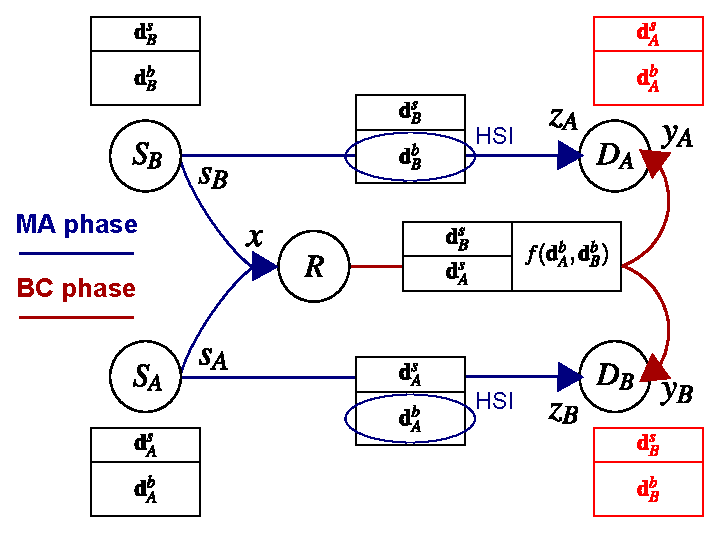
\includegraphics[width=0.6\columnwidth]{fig/2-SRN-sc_principle_BC-TWT_v4}
\caption{Symmetric WBN model with half-duplex constraint and 2-phase communication.\label{fig:CTUpp_Information_flows}}
\end{figure}

\begin{figure*}
\begin{centering}
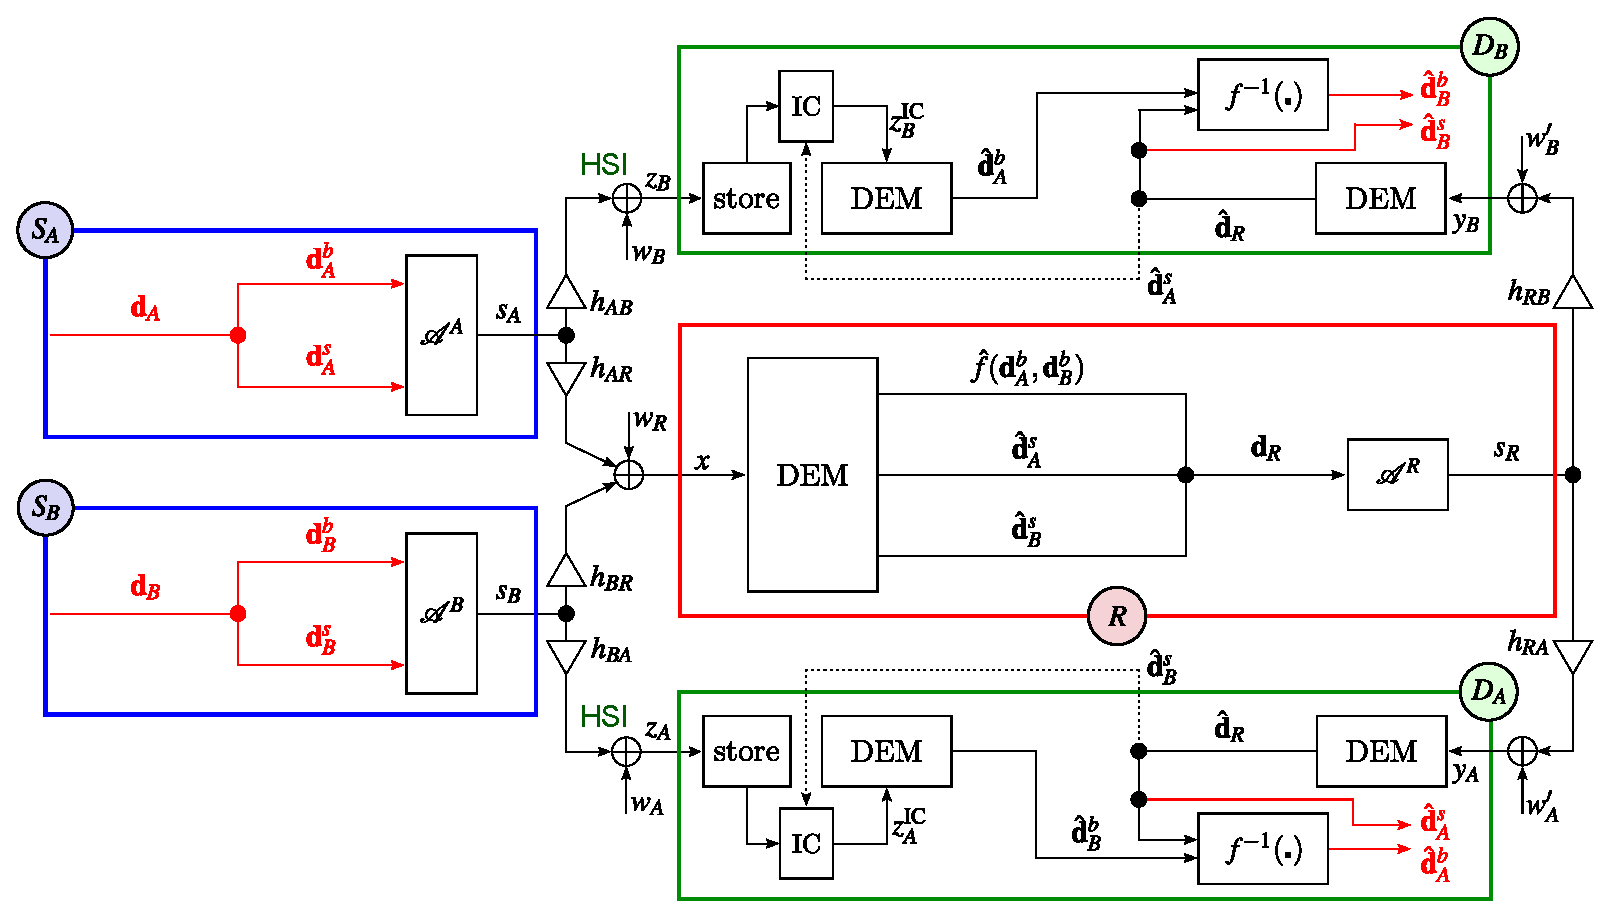
\includegraphics[width=1\textwidth]{fig/butterfly-2level_processing_principleTWC-uncoded}
\par\end{centering}
\caption{Relaying scheme for the uncoded WBN
system. DEM stands for a hard decision demodulator, IC is the interference
canceler.\label{fig:CTUpp_Information-flow-uncoded-block-scheme}}
\end{figure*}
\begin{figure*}
\centering{}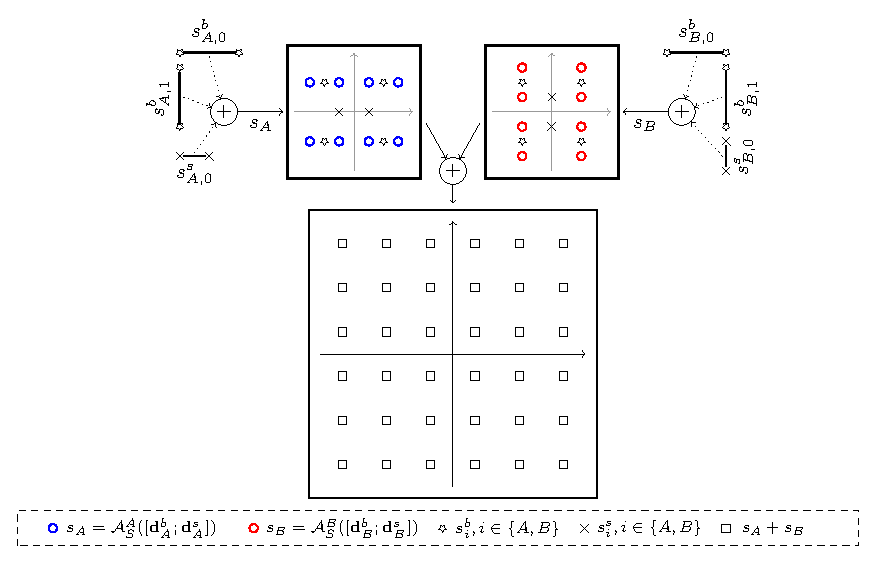
\includegraphics[width=0.8\textwidth]{fig/d2_1}\caption{Source constellation design example for $N_{b}=2,\,N_{s}=1$. Resulting
constellations are depicted as blue circles ($S_{A}$ output constellation),
red circles ($S_{B}$ output constellation) and squares (received
superimposed constellation at $R$). Hierarchical function is $f\left(\mathbf{d}_{A}^{b},\,\mathbf{d}_{B}^{b}\right)=\mathbf{d}_{A}^{b}\oplus\mathbf{d}_{B}^{b}$.\label{fig:CTUpp_ConstellationDesignExample} }
\end{figure*}
\begin{figure*}
\begin{centering}
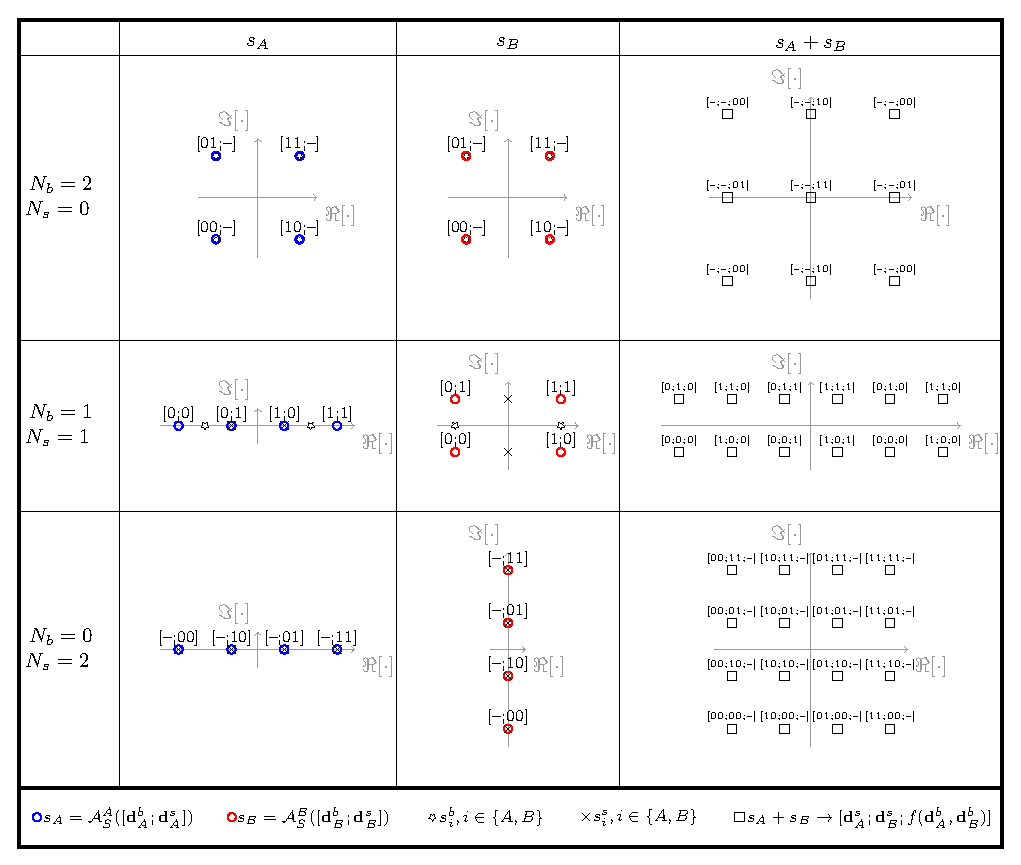
\includegraphics[width=1\textwidth]{fig/const_all_2}
\par\end{centering}

\caption{Proposed constellation design for $\left(N_{b},N_{s}\right)=\left\{ \left(2,0\right);\left(1,1\right);\left(0,2\right)\right\} $.\label{fig:CTUpp_ConstellationDesign_NbNs2} }
\end{figure*}

\begin{figure}
\centering{}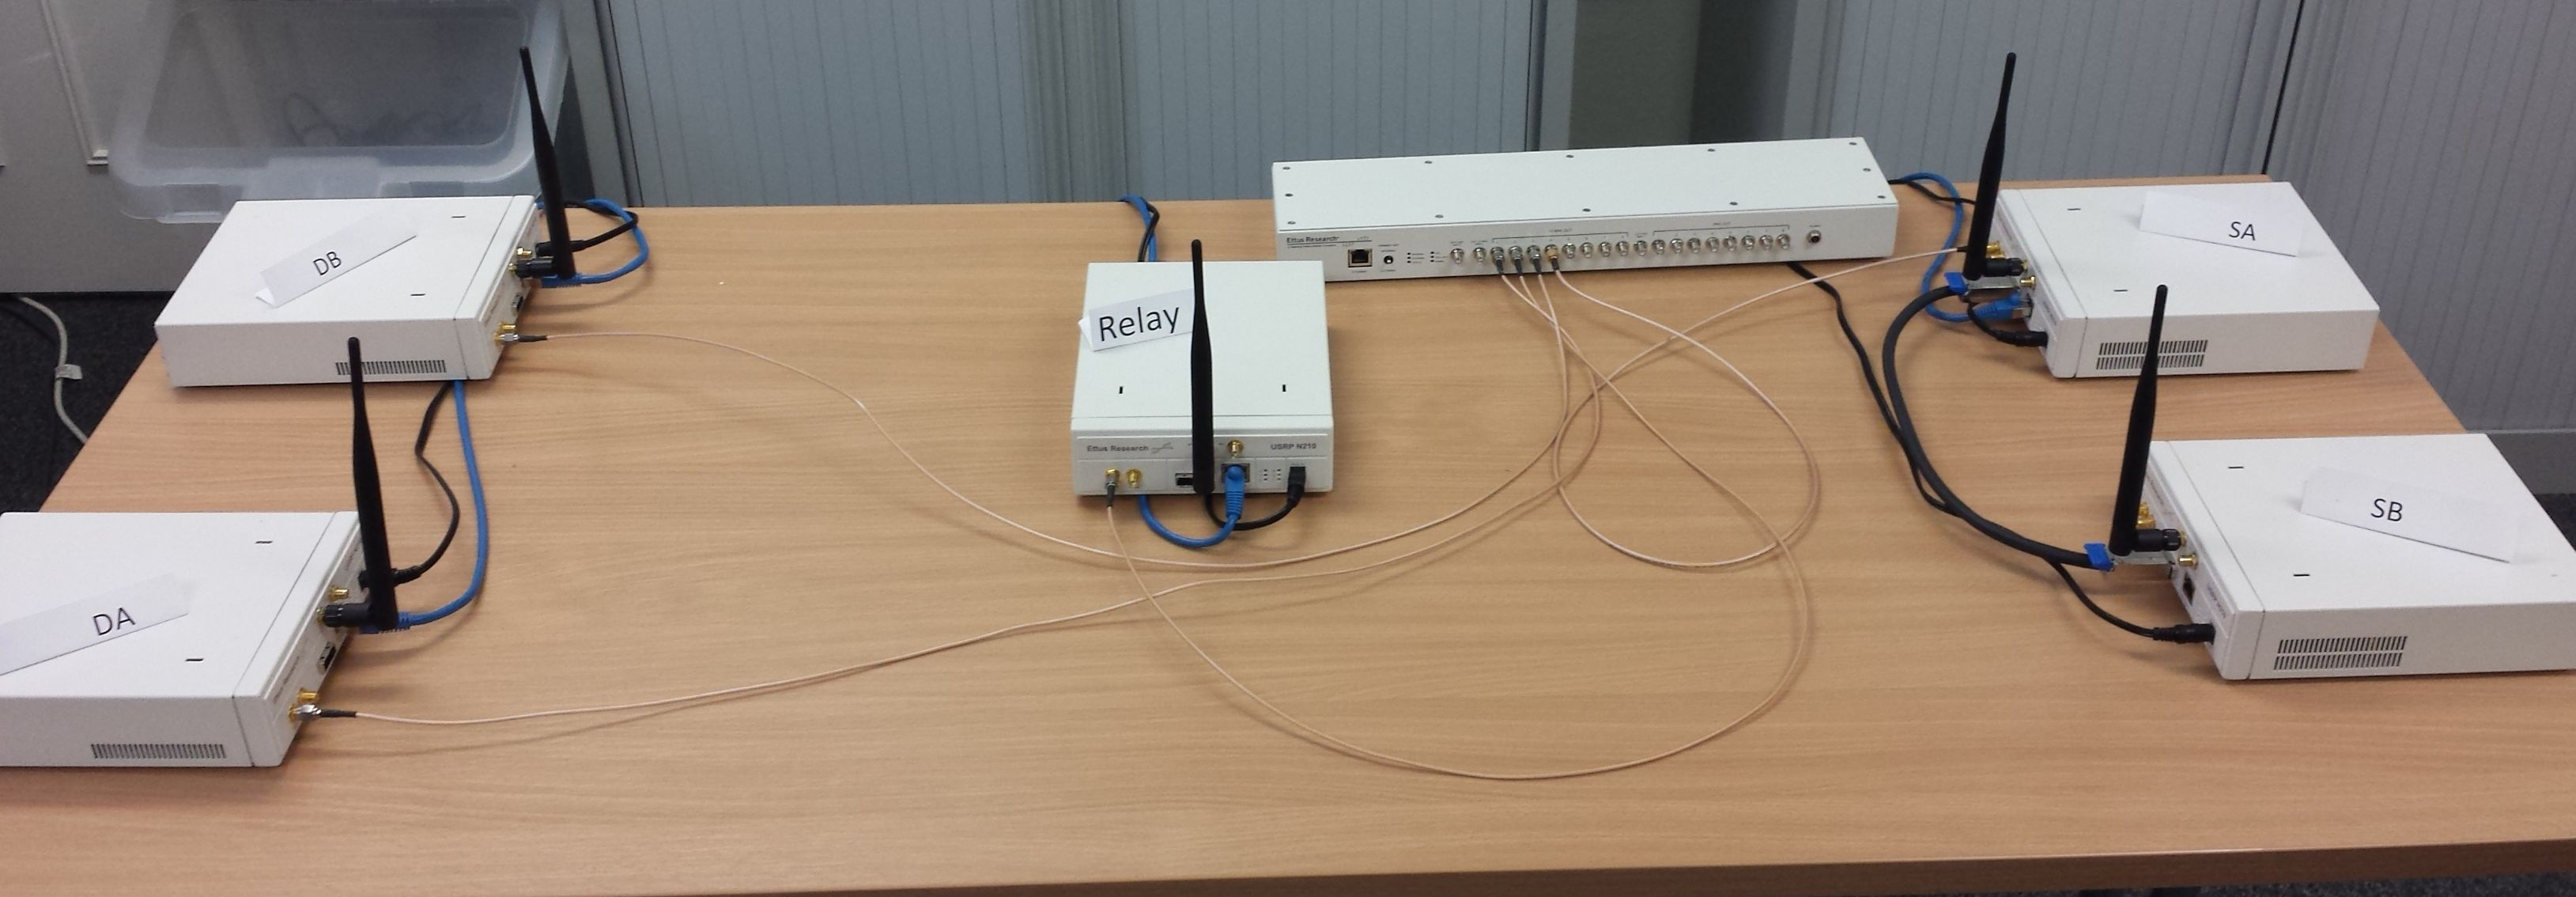
\includegraphics[width=0.95\columnwidth]{fig/20150109_143009}\caption{Setup for HW evaluation (Ettus Research
USRPs). Source transmissions are prerotated \cite{Koike-Popovski-Tarokh_2009a,Zhang-Liew_2010,Anxin-Yuan-Kayama_2008}
to imitate the AWGN channel conditions (as used in the numerical evaluation).
To allow a strict control of HSI channels SNR in the HW
setup, the HSI channels are emulated by adding a Gaussian noise to
the respective source signal and the resulting emulated HSI is passed
to destinations via UDP. This also avoids the problem of node visibility
where direct links $S_{A}\rightarrow D_{A}$ and $S_{B}\rightarrow D_{B}$
exist in the laboratory environment.\label{fig:CTUpp_HW_setup}}
\end{figure}

\begin{figure}
\begin{centering}
\hspace*{-0.04\columnwidth}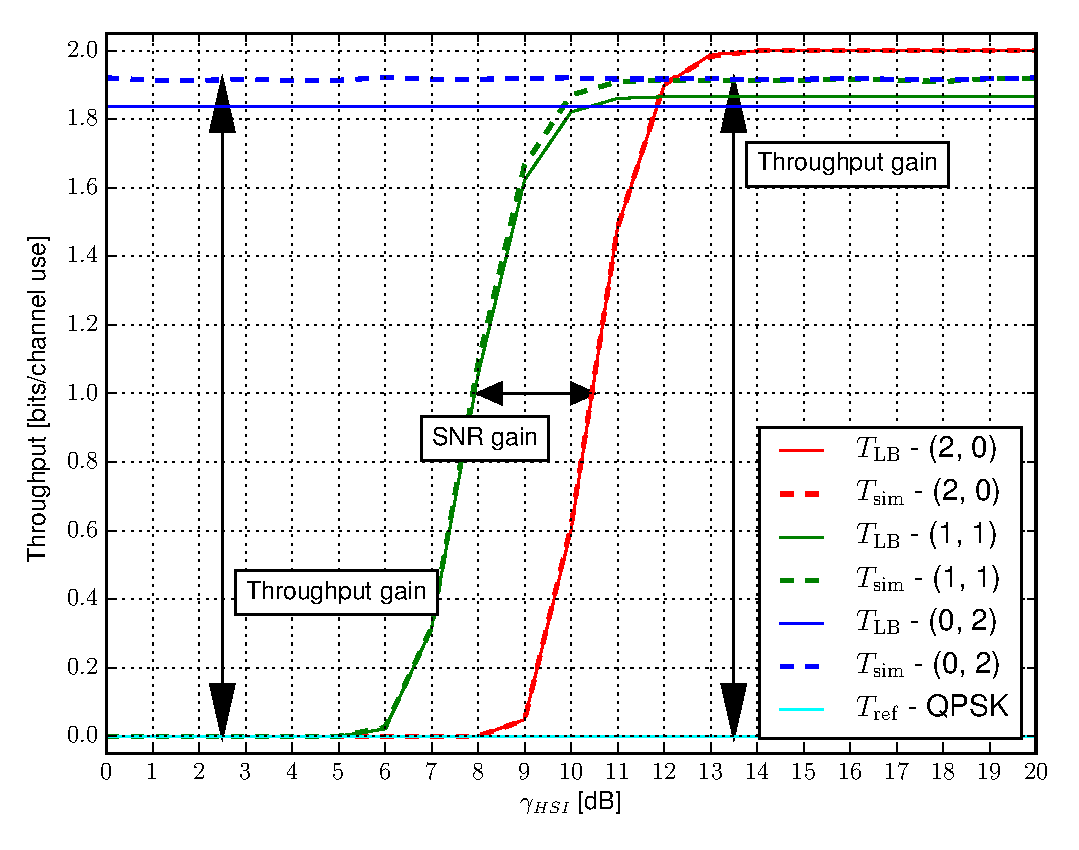
\includegraphics[width=0.95\columnwidth]{fig/Throughput_HSI_XOR_MAC16_BC20_N2}
\par\end{centering}

\caption{Comparison of throughput as a function of $\gamma_{{\rm {HSI}}}$
for $\gamma_{{\rm {MAC}}}=16\,\mathrm{dB},\,\gamma_{{\rm {BC}}}=20\,\mathrm{dB}$
and given $(N_{b},N_{s})$. \label{fig:CTUpp_Throughput16_20}}
\end{figure}
\begin{figure}
\begin{centering}
\hspace*{-0.04\columnwidth}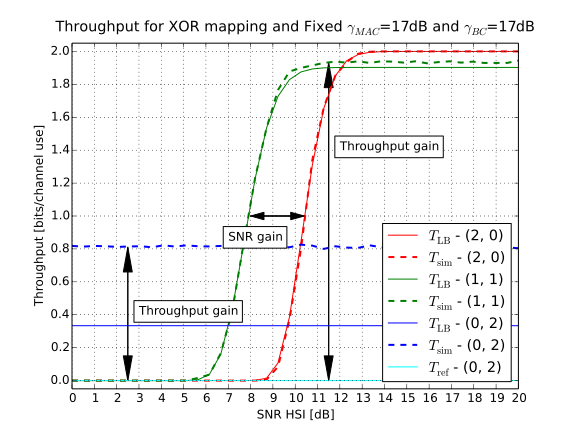
\includegraphics[width=0.95\columnwidth]{fig/Throughput_HSI_XOR_MAC17_BC17_N2}
\par\end{centering}

\caption{Comparison of throughput as a function of $\gamma_{{\rm {HSI}}}$
for $\gamma_{{\rm {MAC}}}=17\,\mathrm{dB},\,\gamma_{{\rm {BC}}}=17\,\mathrm{dB}$
and given $(N_{b},N_{s})$.\label{fig:CTUpp_Throughput17_17}}
\end{figure}
\begin{figure}
\begin{centering}
\hspace*{-0.04\columnwidth}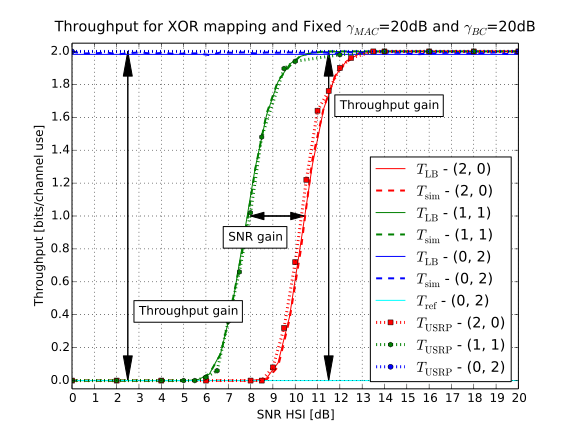
\includegraphics[width=0.95\columnwidth]{fig/Throughput_HSI_XOR_MAC20_BC20_N2}
\par\end{centering}

\caption{Comparison of throughput as a function of $\gamma_{{\rm {HSI}}}$
for $\gamma_{{\rm {MAC}}}=20\,\mathrm{dB},\,\gamma_{{\rm {BC}}}=20\,\mathrm{dB}$
and given $(N_{b},N_{s})$. \label{fig:CTUpp_Throughput20_20}}
\end{figure}
\begin{figure}
\begin{centering}
\hspace*{-0.04\columnwidth}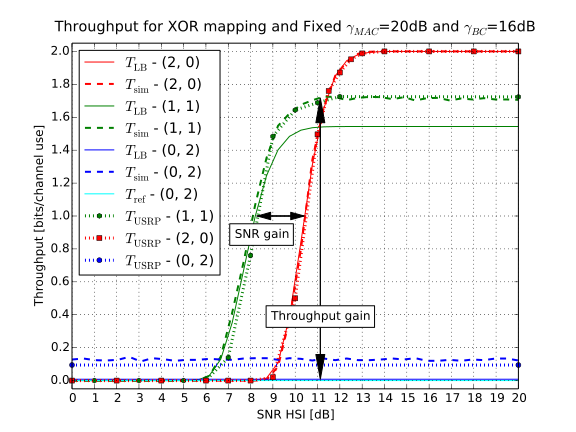
\includegraphics[clip,width=0.95\columnwidth]{fig/Throughput_HSI_XOR_MAC20_BC16_N2}
\par\end{centering}

\caption{Comparison of throughput as a function of $\gamma_{{\rm {HSI}}}$
for $\gamma_{{\rm {MAC}}}=20\,\mathrm{dB},\,\gamma_{{\rm {BC}}}=16\,\mathrm{dB}$
and given $(N_{b},N_{s})$. \label{fig:CTUpp_Throughput20_16}}
\end{figure}


\begin{figure*}
\begin{centering}
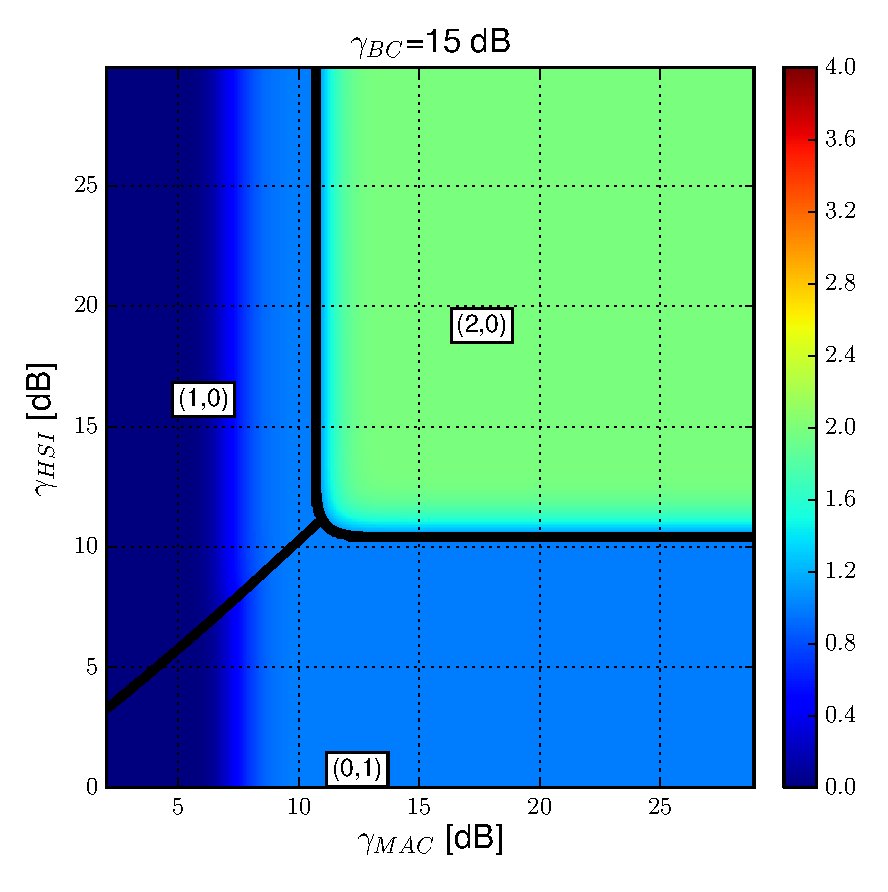
\includegraphics[width=0.45\textwidth]{fig/XOR_map_Througput_BC15}\quad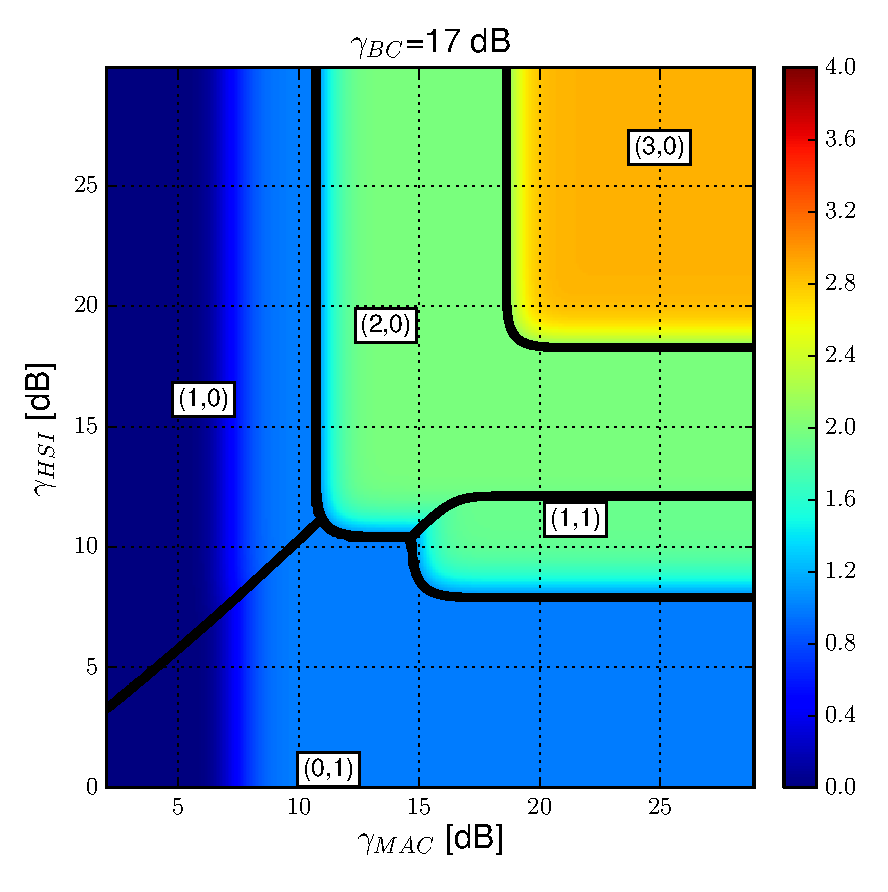
\includegraphics[width=0.45\textwidth]{fig/XOR_map_Througput_BC17}
\par\end{centering}

\centering{}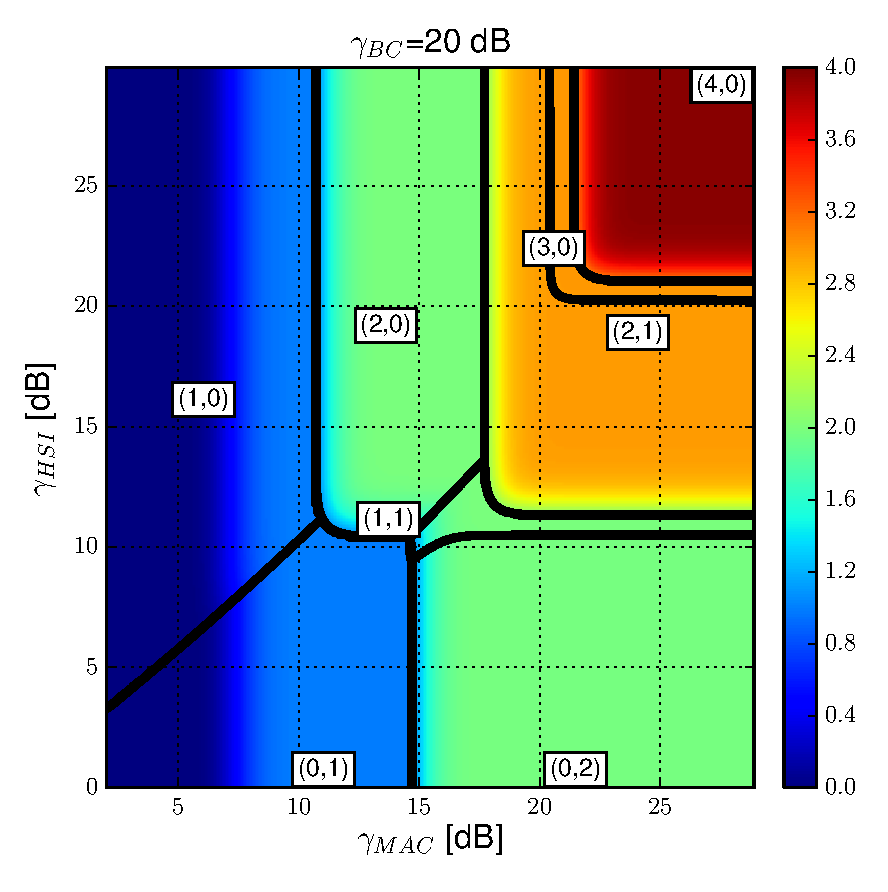
\includegraphics[width=0.45\textwidth]{fig/XOR_map_Througput_BC20}\quad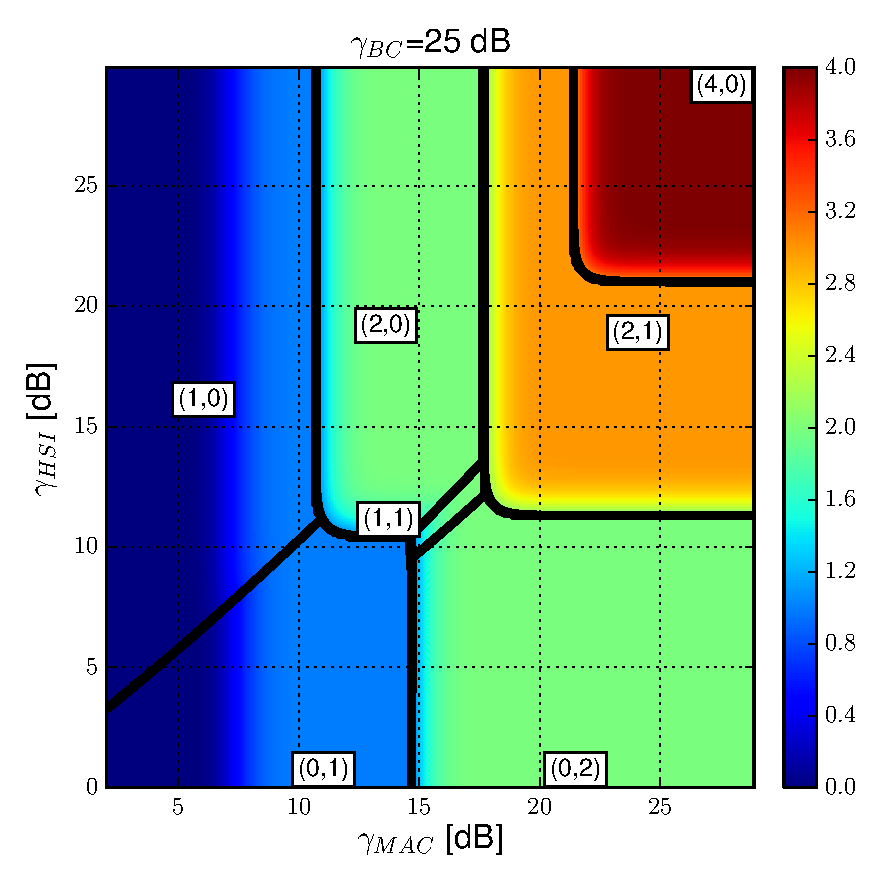
\includegraphics[width=0.45\textwidth]{fig/XOR_map_Througput_BC25}\caption{Throughput performance $T_{\mathrm{LB}}$ and SNR mapping regions
(including the optimal const. parameters ($N_{b}^{{\rm I}},\,N_{s}^{{\rm I}}$))
for $\gamma_{{\rm {BC}}}\in\{15\,\mathrm{dB},\,17\,\mathrm{dB},20\,\mathrm{dB},25\,\mathrm{dB}\}$.\label{fig:CTUpp_SNR_map_BC15-17-20-25}}
\end{figure*}
\begin{figure*}
\centering{}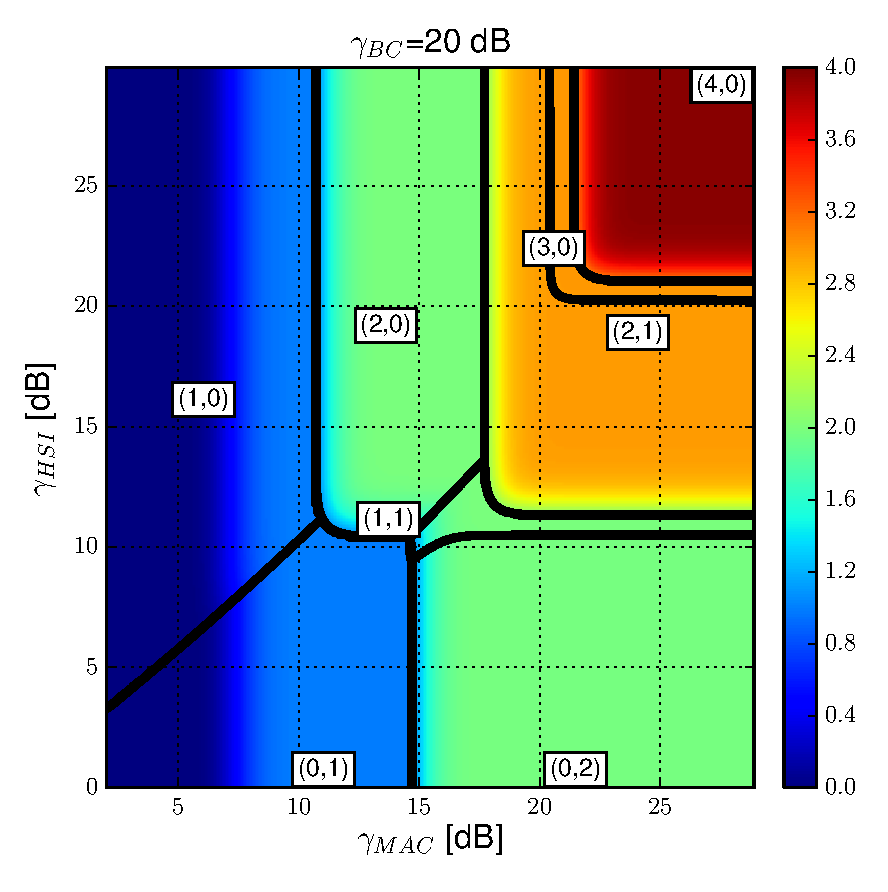
\includegraphics[width=0.48\textwidth]{fig/XOR_map_Througput_BC20}\quad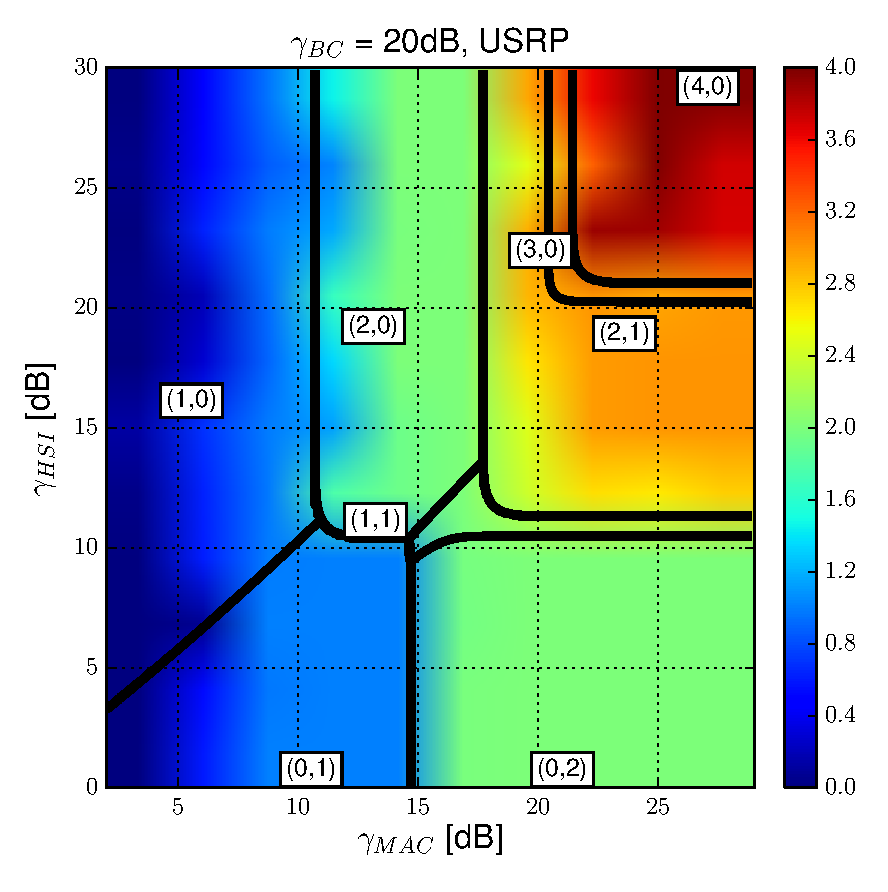
\includegraphics[width=0.48\textwidth]{fig/XOR_map_Througput_USRP_BC20}\caption{Comparison of $T_{\mathrm{LB}}$ and the throughput performance evaluated
in a real world adaptive HW setup ($T_{\mathrm{USRP}}$) for $\gamma_{{\rm {BC}}}=20\,\mathrm{dB}$.
The SNR mapping regions (including the optimal const. parameters ($N_{b}^{{\rm I}},\,N_{s}^{{\rm I}}$))
used in the HW evaluation are also emphasized in the figure.\label{fig:CTUpp_SNR_map_BC20_USRP}}
\vspace*{-4ex}
\end{figure*}

\begin{figure*}
\begin{centering}
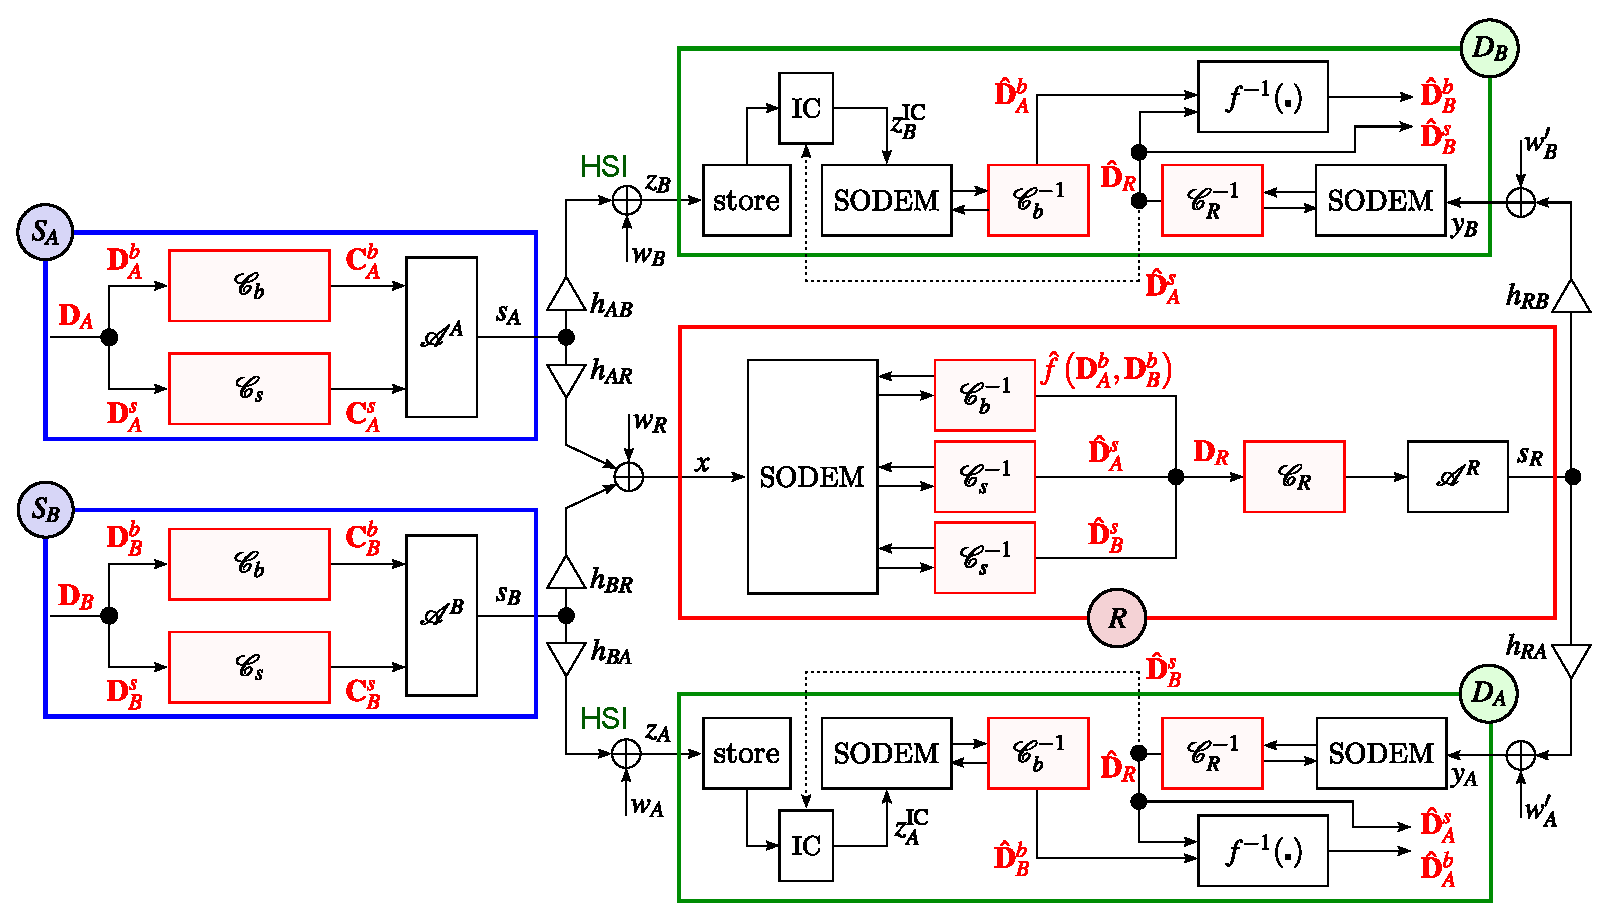
\includegraphics[width=1\textwidth]{fig/butterfly-2level_processing_principleTWC-coded}
\par\end{centering}

\caption{Relaying scheme in the encoded WBN system. SODEM stands for a soft-output
demodulator, IC is the interference canceler. The channel encoders/decoders
which are appended to the uncoded system are emphasized. \label{fig:CTUpp_Information-flow-coded-block-scheme}}
\end{figure*}

\begin{figure*}
\begin{centering}
\hspace*{-1.5em}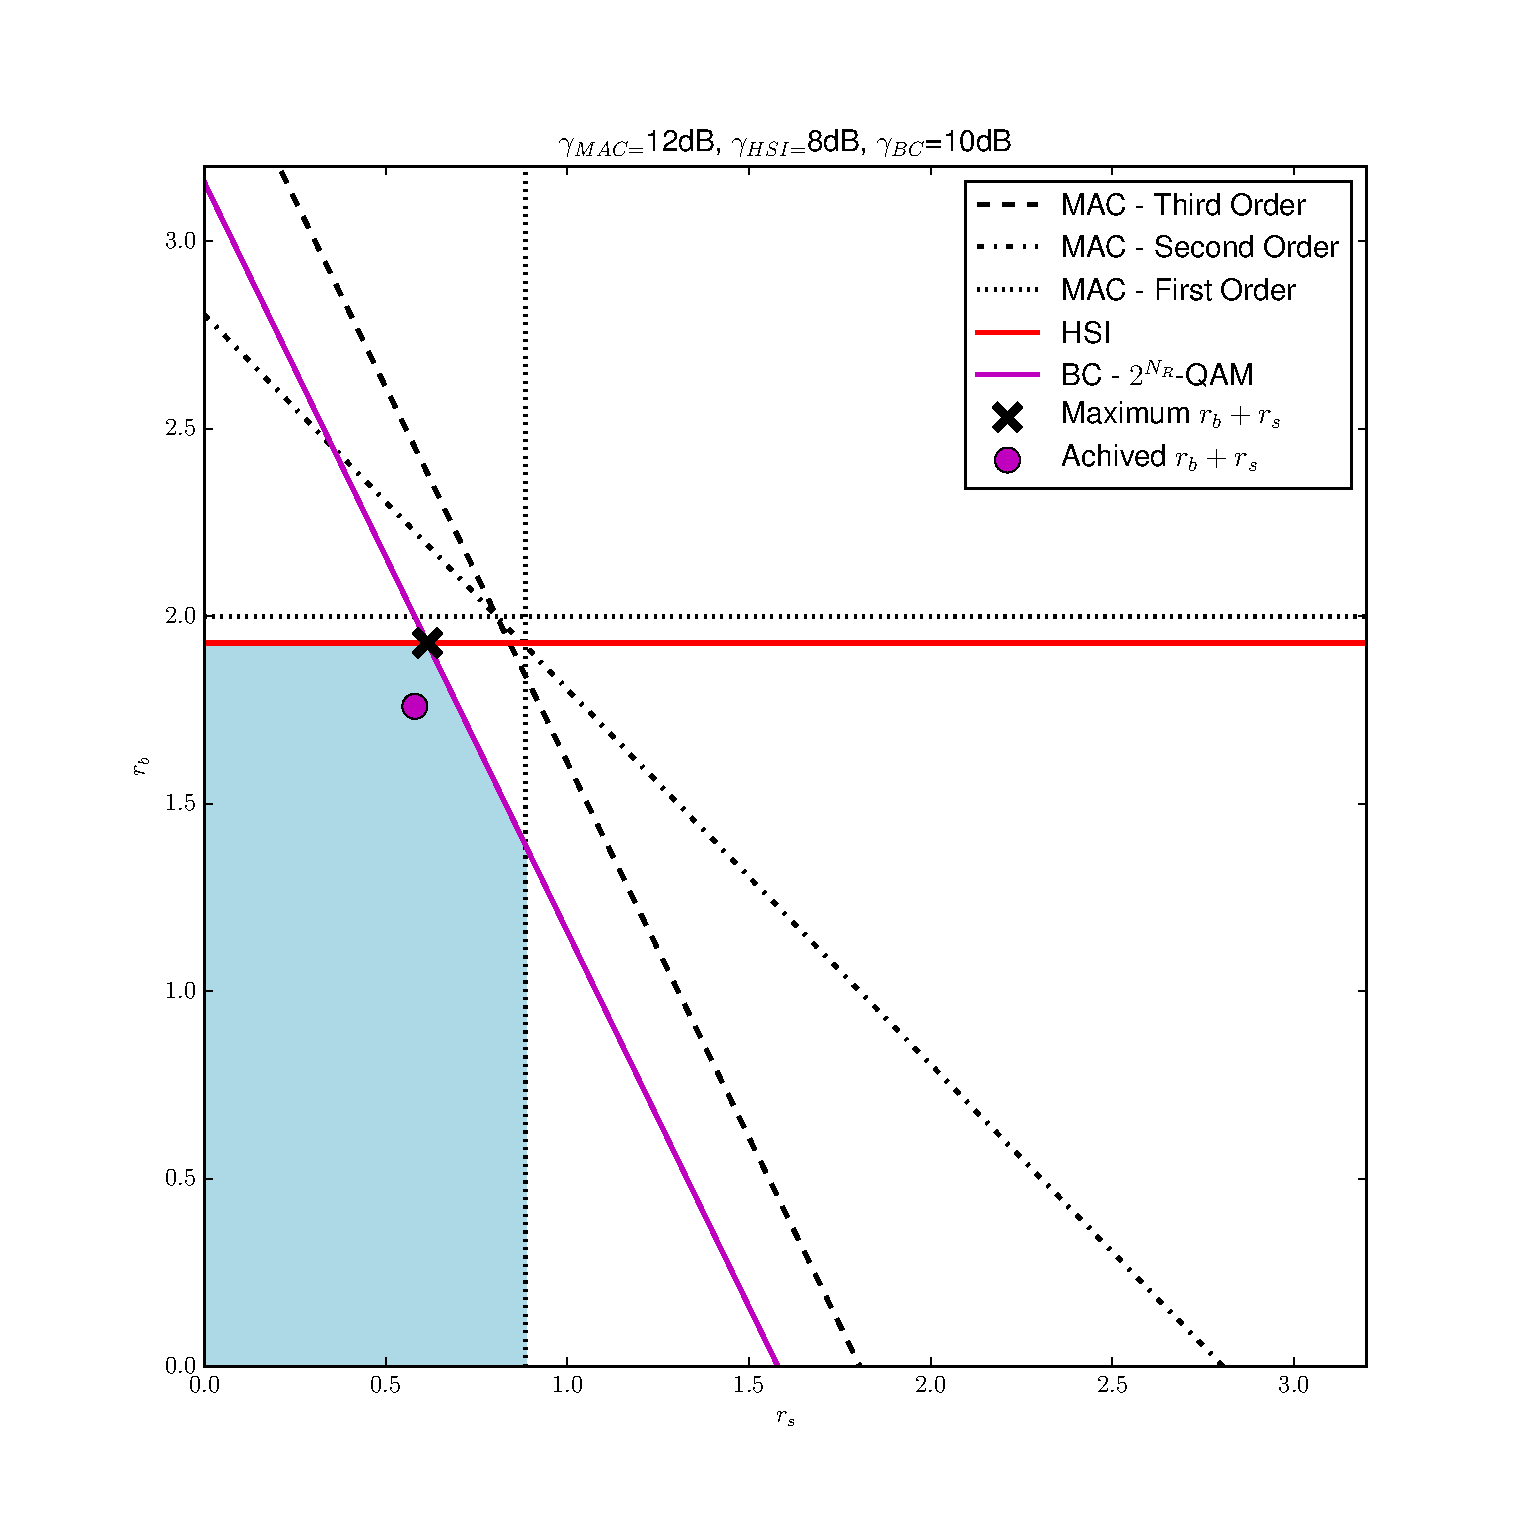
\includegraphics[width=0.7\columnwidth]{fig/Rate_Regions_XOR_map_BC10_MAC12_HSI8}
\par\end{centering}

\begin{centering}
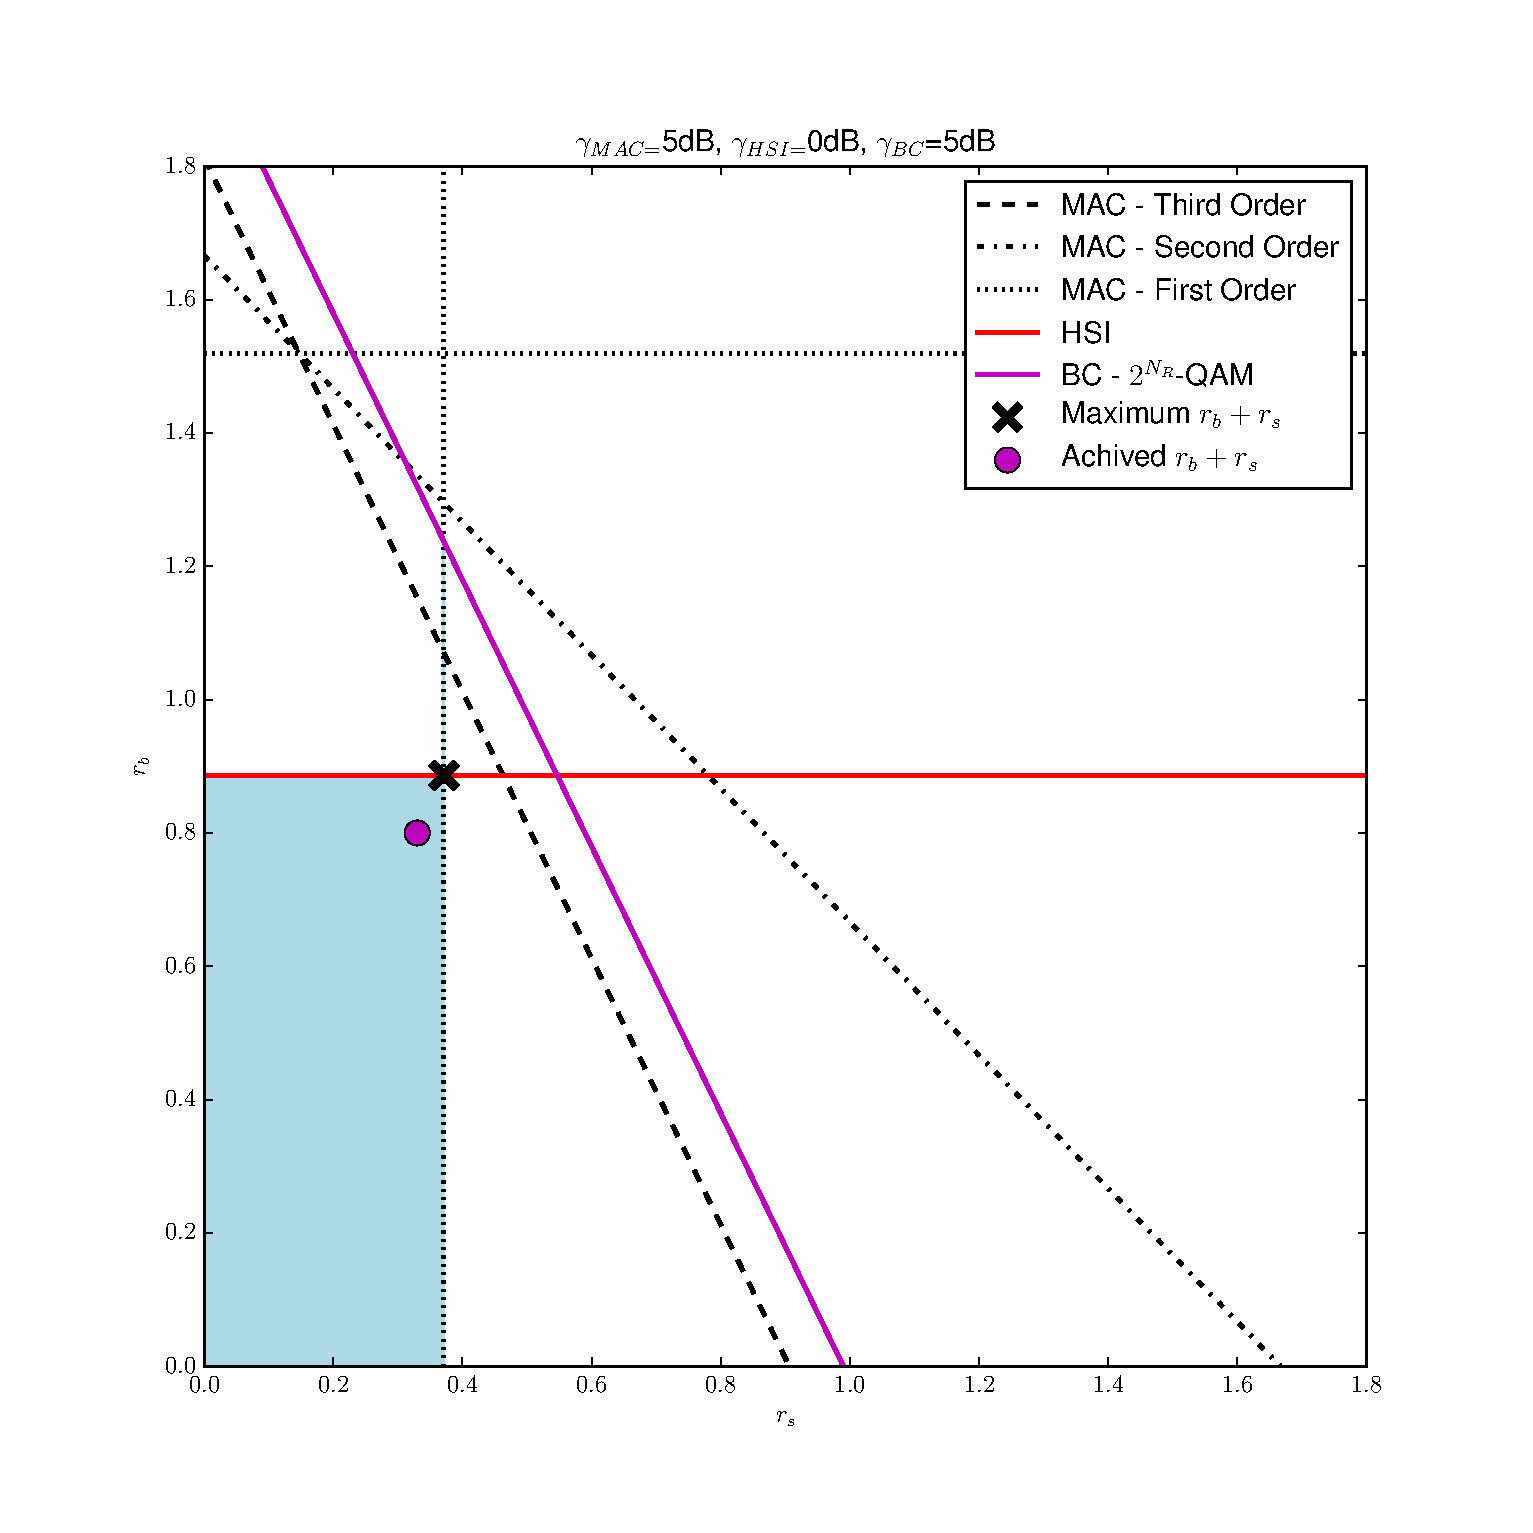
\includegraphics[width=0.7\textwidth]{fig/Rate_Regions_XOR_map_BC5_MAC5_HSI0}
\par\end{centering}

\caption{Numerically evaluated cut-set bounds (mutual information for finite
input constellations) for $(N_{b}=2,N_{s}=1)$ source constellations
and $16$-QAM at the relay. The particular SNR conditions are available
in the titles of both sub-figures.\label{fig:CTUpp_CSB_eval}}
\end{figure*}

\begin{figure*}
\centering{}\includegraphics[width=0.45\textwidth]{fig/Adaptive_Maps_overall_BC_7\lyxdot 5}~~~\includegraphics[width=0.45\textwidth]{fig/Adaptive_Maps_overall_BC_15\lyxdot 0}\caption{Maximal encoded system throughput $T_{C}^{\mathrm{max}}$ for $\gamma_{{\rm {BC}}}=7.5\,\mathrm{dB}$
and $\gamma_{{\rm {BC}}}=15\,\mathrm{dB}$.\label{fig:CTUpp_Coded_SNR_map} }
\end{figure*}
\begin{figure*}
\centering{}\includegraphics[width=0.45\textwidth]{fig/XOR_map_Througput_coding_Gain7\lyxdot 5}~~~\includegraphics[width=0.45\textwidth]{fig/XOR_map_Througput_coding_Gain15\lyxdot 0}\caption{Throughput enhancement $\Delta T_{C}=T_{C}^{\mathrm{max}}-T_{\mathrm{LB}}$
{[}bits/channel use{]} of the coded over uncoded WBN system for $\gamma_{{\rm {BC}}}=7.5\,\mathrm{dB}$
and $\gamma_{{\rm {BC}}}=15\,\mathrm{dB}$. Note that $0.75\leq\Delta T_{C}\leq2$
in the analyzed range of channel SNRs.\label{fig:CTUpp_Coded_ThroughputGain}}
\end{figure*}

\begin{figure}
\begin{centering}
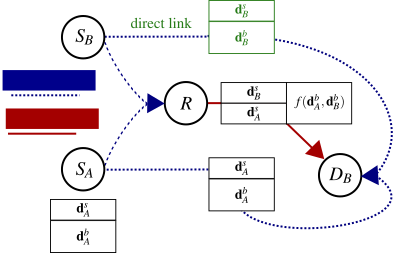
\includegraphics[width=0.75\columnwidth]{fig/2-SRN-sc_principle_BC-TWT_directLink}
\par\end{centering}

\centering{}\caption{Direct channel at destination $D_{B}$ in the robustness analysis
(likewise, a direct channel is assumed to be present also at $D_{A}$).\label{fig:CTUpp_DirectChannel}}
\end{figure}

\begin{figure*}
\centering{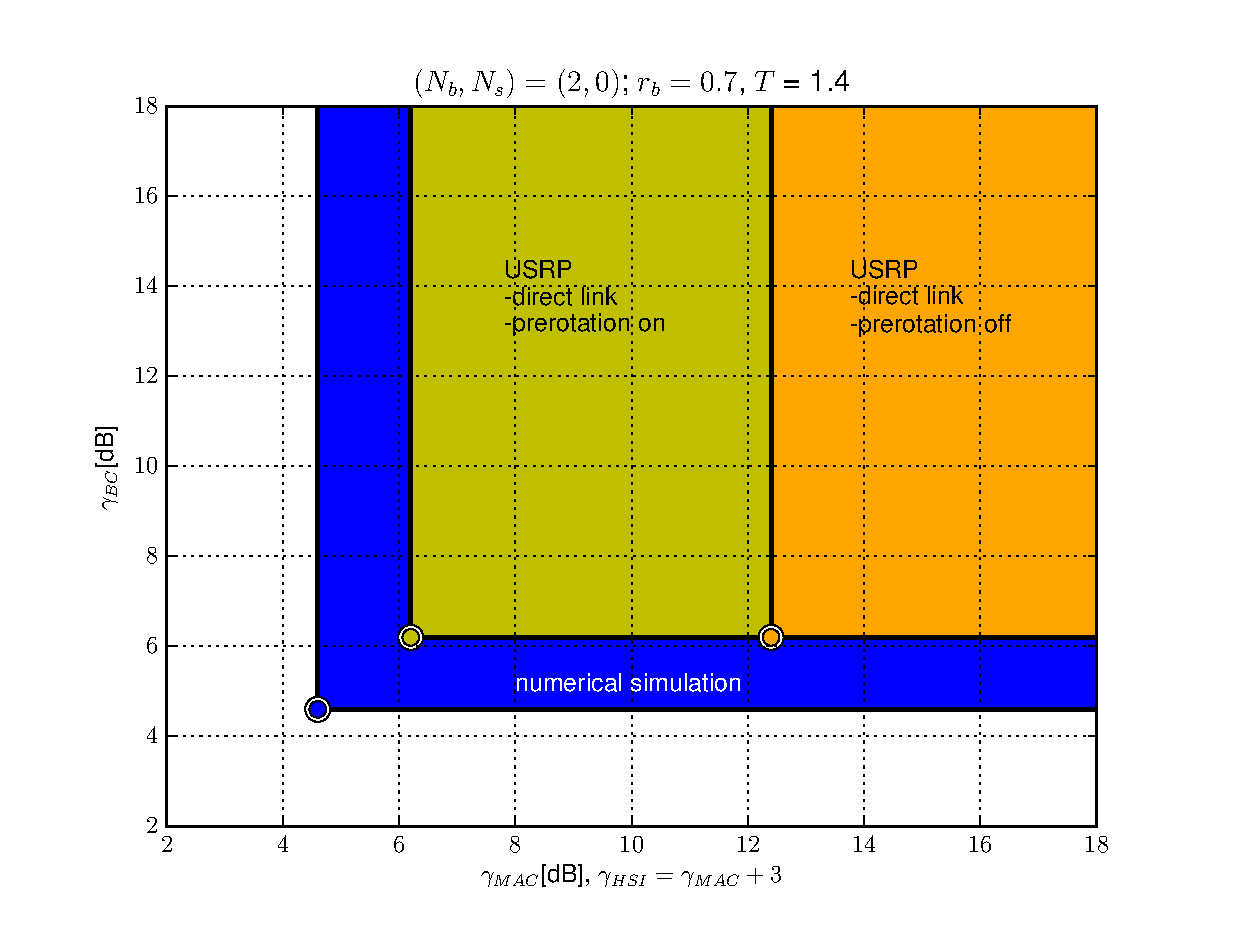
\includegraphics[width=1\textwidth]{fig/Robust_20}
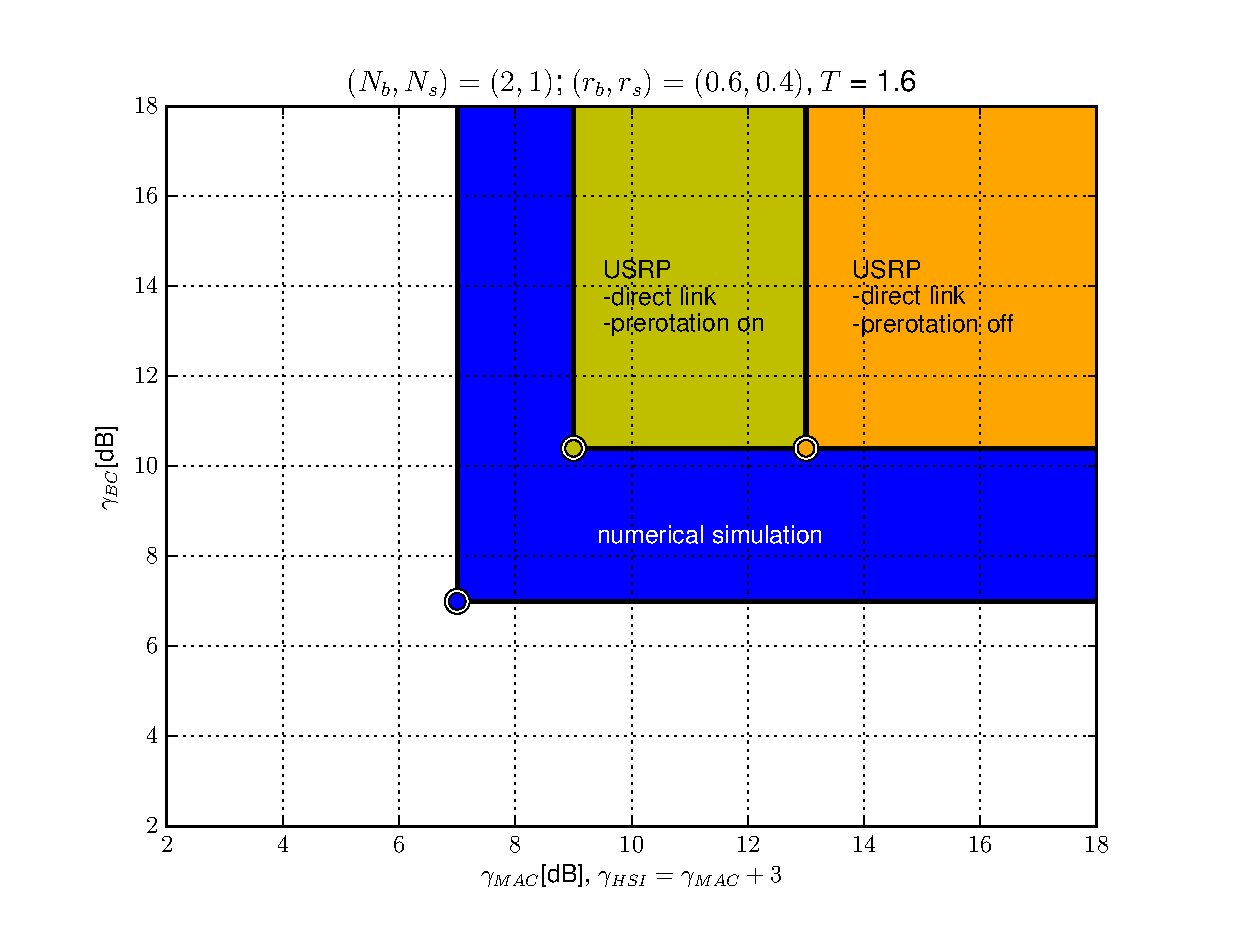
\includegraphics[width=1\textwidth]{fig/Robust_21}}
\caption{Robustness analysis for two fixed $(N_{b},N_{s},r_{b},r_{s})$ scenarios.
\label{fig:CTUpp_Robustenss_analysis}}
\end{figure*}
\section*{Availability of Data and Materials}

\bibliographystyle{bmc_template/bmc-mathphys}
\bibliography{bib/bib,bib/uricar,bib/uricar-papers,bib/uricar-books,bib/sykora,bib/books}

\end{backmatter}
\end{document}
